\documentclass[10pt]{article}
\usepackage[english]{babel}
\usepackage[utf8x]{inputenc}
\usepackage[T1]{fontenc}
\usepackage{amsmath}
\usepackage{amssymb}
\usepackage{graphicx}
\usepackage[colorlinks=true, allcolors=black, hypertexnames=false]{hyperref}
\usepackage{epsfig,amsfonts}
\usepackage{authblk}
\usepackage{subfig}
\usepackage{setspace}
\usepackage{hypcap}
\usepackage{lscape}
\usepackage{lineno}
\usepackage{latexsym,color,soul,xspace,tabularx}
\usepackage{booktabs}
\usepackage{multirow,multicol}
\usepackage{pdflscape}
\pagestyle{myheadings}
\usepackage{bm}
\usepackage{bbm}
\usepackage{adjustbox}
\usepackage{xr}
\makeatletter
\newcommand*{\addFileDependency}[1]{% argument=file name and extension
  \typeout{(#1)}
  \@addtofilelist{#1}
  \IfFileExists{#1}{}{\typeout{No file #1.}}
}
\makeatother
\newcommand*{\myexternaldocument}[1]{%
    \externaldocument{#1}%
    \addFileDependency{#1.tex}%
    \addFileDependency{#1.aux}%
}
\myexternaldocument{Supplementary}
\usepackage{textgreek}

\def\eq#1{(\ref{#1})}
\def\pdf{p.d.f.\ } \def\cdf{c.d.f.\ }
\def\pdfs{p.d.f.s} \def\cdfs{c.d.f.s}
\def\mgf{m.g.f.\ } \def\mgfs{m.g.f.s\ }
\def\ci{\perp   \perp}  
\def\beginmat{ \left( \begin{array} }
\def\endmat{ \end{array} \right) }
\def\diag{{\rm diag}}
\def\log{{\rm log}}
\def\tr{{\rm tr}}
\def\cond{\, | \,}
\newcommand*\diff{\mathop{}\!\mathrm{d}}

\def\dsum{\displaystyle\sum}
\def\dint{\displaystyle\int}
\def\dsup{\displaystyle\sup}
\def\dinf{\displaystyle\inf}
\def\dmin{\displaystyle\min}
\def\dlim{\displaystyle\lim}

\newcommand{\me}{\mathrm{e}}
\newcommand{\supp}{\operatorname{supp}}
\newcommand{\abs}[1]{\left|#1\right|}
\newcommand{\comment}[1]{{\em #1}}
\newcommand{\ba}{\mathbf{a}}
\newcommand{\bb}{\mathbf{b}}
\newcommand{\bc}{\mathbf{c}}
\newcommand{\be}{\mathbf{e}}
\newcommand{\bg}{\mathbf{g}}
\newcommand{\bl}{\mathbf{l}}
\newcommand{\bs}{\mathbf{s}}
\newcommand{\bq}{\mathbf{q}}
\newcommand{\bk}{\mathbf{k}}
\newcommand{\bv}{\mathbf{v}}
\newcommand{\bx}{\mathbf{x}}
\newcommand{\by}{\mathbf{y}}
\newcommand{\bz}{\mathbf{z}}
\newcommand{\bh}{\mathbf{h}}
\newcommand{\bu}{\mathbf{u}}
\newcommand{\bfm}{\mathbf{m}}
\newcommand{\bw}{\mathbf{w}}
\newcommand{\w}{\mathbf{w}}
\newcommand{\bp}{\mathbf{p}}
\newcommand{\bK}{\mathbf{K}}
\newcommand{\bV}{\mathbf{V}}
\newcommand{\bA}{\mathbf{A}}
\newcommand{\bB}{\mathbf{B}}
\newcommand{\bC}{\mathbf{C}}
\newcommand{\bX}{\mathbf{X}}
\newcommand{\bY}{\mathbf{Y}}
\newcommand{\bE}{\mathbf{E}}
\newcommand{\bG}{\mathbf{G}}
\newcommand{\bH}{\mathbf{H}}
\newcommand{\bP}{\mathbf{P}}
\newcommand{\bQ}{\mathbf{Q}}
\newcommand{\bR}{\mathbf{R}}
\newcommand{\bW}{\mathbf{W}}
\newcommand{\bM}{\mathbf{M}}
\newcommand{\bU}{\mathbf{U}}
\newcommand{\bZ}{\mathbf{Z}}
\newcommand{\bD}{\mathbf{D}}
\newcommand{\bI}{\mathbf{I}}
\newcommand{\bS}{\mathbf{S}}
\newcommand{\T}{\intercal}
\newcommand{\wt}{\widetilde}
\newcommand{\wh}{\widehat}

\newcommand{\E}{\mathbb{E}}
\newcommand{\V}{\mathbb{V}}

\newcommand{\bbE}{\mathbb{E}}
\newcommand{\bbV}{\mathbb{V}}
\newcommand{\N}{\mathcal{N}}

\newcommand{\bepsilon}{\boldsymbol\epsilon}
\newcommand{\bvarepsilon}{\boldsymbol\varepsilon}
\newcommand{\bbeta}{\boldsymbol\beta}
\newcommand{\bsigma}{\boldsymbol\sigma}
\newcommand{\tbbeta}{{\tilde{\boldsymbol\beta}}}
\newcommand{\tbeta}{{\tilde{\beta}}}
\newcommand{\bgamma}{\boldsymbol\gamma}
\newcommand{\bdelta}{\boldsymbol\delta}
\newcommand{\btheta}{\boldsymbol\theta}
\newcommand{\bpsi}{\boldsymbol\psi}
\newcommand{\bphi}{\boldsymbol\phi}
\newcommand{\brho}{\boldsymbol\rho}
\newcommand{\balpha}{\boldsymbol\alpha}
\newcommand{\bmu}{\boldsymbol\mu}
\newcommand{\bomega}{\boldsymbol\omega}
\newcommand{\btau}{\boldsymbol\tau}
\newcommand{\bDelta}{\boldsymbol\Delta}
\newcommand{\bOmega}{\boldsymbol\Omega}
\newcommand{\bSigma}{\boldsymbol\Sigma}
\newcommand{\bLambda}{\boldsymbol\Lambda}
\newcommand{\bTheta}{\boldsymbol\Theta}
\newcommand{\at}[2][]{#1|_{#2}}
\newcommand{\red}[1]{\textcolor{red}{#1}}
\newcommand{\blue}[1]{\textcolor{blue}{#1}}

\topmargin 0.0cm
\oddsidemargin 0.5cm
\evensidemargin 0.5cm
\textwidth 16cm 
\textheight 21cm

\newcommand{\edit}[2]{\sout{#1}\textcolor{red}{\xspace#2}}
\newcommand{\black}{\textcolor{black}}

\newcolumntype{R}[2]{%
    >{\adjustbox{angle=#1,lap=\width-(#2)}\bgroup}%
    l%
    <{\egroup}%
}
\newcommand*\rot{\multicolumn{1}{R{90}{1em}}}
\newcolumntype{P}[1]{>{\centering\arraybackslash}p{#1}}

% Bold the 'Figure #' in the caption and separate it with a period
% Captions will be left justified
\usepackage[labelfont=bf,labelsep=period,justification=justified]{caption}
\allowdisplaybreaks
\renewcommand\thesubfigure{(\alph{subfigure})}
\bibliographystyle{plos2015}
\usepackage{cite}

% Remove brackets from numbering in List of References
\makeatletter
\renewcommand{\@biblabel}[1]{\quad#1.}
\makeatother

%% END MACROS SECTION

%%%%%%%%%%%%%%%%%%%%%%%%%%%%%%%%%%%%%%%%%%%%%%%%%%%
%%%%%%%%%%%%%%%%%%%%%%%%%%%%%%%%%%%%%%%%%%%%%%%%%%%
%%%%%%%%%%%%%%%%%%%%%%%%%%%%%%%%%%%%%%%%%%%%%%%%%%%

\begin{document}

\linenumbers
\begin{flushleft}
{\Large
\textbf{Pathway Analysis within Multiple Human Ancestries Reveals Novel Signals for Epistasis in Complex Traits}
}
\newline
% Insert Author names, affiliations and corresponding author email.
\\
Michael C. Turchin\textsuperscript{1,2,$\dagger$}, Gregory Darnell\textsuperscript{2,3}, Lorin Crawford\textsuperscript{2,4,*,$\dagger$}, and Sohini Ramachandran\textsuperscript{1,2,*,$\dagger$} 
\\
\bigskip
\bf{1} Department of Ecology and Evolutionary Biology, Brown University, Providence, RI, USA
\\
\bf{2} Center for Computational Molecular Biology, Brown University, Providence, RI, USA
\\
\bf{3} Institute for Computational and Experimental Research in Mathematics (ICERM), Brown University, Providence, RI, USA
\\
\bf{4} Microsoft Research New England, Cambridge, MA, USA
\\
\bigskip
*: Authors Contributed Equally\\
$\dagger$ Corresponding E-mail: michael\_turchin@brown.edu; lcrawford@microsoft.com; sramachandran@brown.edu 
\end{flushleft}

%%%%%%%%%%%%%%%%%%%%%%%%%%%%%%%%%%%%%%%%%%%%%%%%%%%

\section*{Abstract}\label{MAPITR-Abstract} 

Genome-wide association (GWA) studies have identified thousands of significant genetic associations in humans across a number of complex traits. However, the majority of these studies focus on linear additive relationships between genotypic and phenotypic variation. Epistasis, or non-additive genetic interactions, has been identified as a major driver of both complex trait architecture and evolution in multiple model organisms; yet, this same phenomenon is not considered to be a significant factor underlying human complex traits. There are two possible reasons for this assumption. First, most large GWA studies are conducted solely with European cohorts; therefore, our understanding of broad-sense heritability for many complex traits is limited to just one ancestry group. Second, current epistasis mapping methods commonly identify significant genetic interactions by exhaustively searching across all possible pairs of SNPs. In these frameworks, estimated epistatic effects size are often small and power can be low due to the multiple testing burden. Here, we present a case study that uses a novel region-based mapping approach to analyze sets of variants for the presence of epistatic effects across six diverse subgroups within the UK Biobank. We refer to this method as the ``MArginal ePIstasis Test for Regions'' or MAPIT-R. Even with limited sample sizes, we find a total of 245 pathways within the KEGG and REACTOME databases that are significantly enriched for epistatic effects in height and body mass index (BMI), with 67\% of these pathways being detected within individuals of African ancestry. As a secondary analysis, we introduce a novel region-based ``leave-one-out'' approach to localize pathway-level epistatic signals to specific interacting genes in BMI. Overall, our results indicate that non-European ancestry populations may be better suited for the discovery of non-additive genetic variation in human complex traits --- further underscoring the need for publicly available, biobank-sized datasets of diverse groups of individuals.

%%%%%%%%%%%%%%%%%%%%%%%%%%%%%%%%%%%%%%%%%%%%%%%%%%%

\section*{Introduction}\label{MAPITR-Introduction}

Genome-wide association (GWA) studies are a powerful tool for understanding the genetic architecture of complex traits and phenotypes \cite{Hirschhorn2005,McCarthy2008,Stranger2011,Yang2014,Pasaniuc2017,Visscher2017,Buniello2019,Tam2019}. The most common approach for conducting GWA studies is to use a linear mixed model to test for statistical associations between individual genetic variants and a phenotype of interest; here, the estimated regression coefficients represent an additive relationship between number of copies of a single-nucleotide polymorphism (SNP) and the phenotypic state. While this approach has produced many statistically significant additive associations, it is less amenable to detecting nonlinear genetic associations that also contribute to a trait's genetic architecture. Epistasis, commonly defined as the nonlinear, or non-additive, interaction between multiple genetic variants, is a well-established phenomenon in a number of model organisms \cite{Lehner2006,Rowe2008,Shao2008,Flint2009,Costanzo2010,He2010,Jarvis2011,Pettersson2011,Bloom2013,Monnahan2015}. Epistasis has also been suggested as a major driver of both phenotypic variation and evolution \cite{Carlborg2004,Carlborg2006,Martin2007,Phillips2008,Moore2009,Zuk2012,Jones2014,Mackay2014}. Still, there remains skepticism and controversy regarding the importance of epistasis in human complex traits and diseases \cite{Hill2008,Crow2010,Yang2010,Aschard2012,Powell2013,Maki-Tanila2014,Wood2014a,Yang2015}. For example, multiple studies have suggested that phenotypic variation can be mainly explained with additive effects \cite{Hill2008,Crow2010,Maki-Tanila2014}; although, this hypothesis has been been challenged recently \cite{Huang2016}. In initial work to locate the  ``missing heritability'' in the human genome --- the discrepancy between larger pedigree-based trait heritability estimates and smaller SNP-based trait heritability estimates using the first wave of human GWA study results \cite{Maher2008,Manolio2009,Eichler2010} --- it was suggested that epistasis may account for a significant portion of this observed discrepancy \cite{Slatkin2009,Zuk2012,Hemani2013}. However, other studies have posited that, for at least some human phenotypes, genetic interactions are unlikely to be a major contributor to total heritability \cite{Yang2015,Wainschtein2019,Roberts2020}.

Algorithmically, detecting statistically significant epistatic signals via genome-wide scans is much more computationally expensive than the the traditional hypothesis-generating GWA framework. GWA tests for additive effects are linear in the number of SNPs, while epistasis scans usually consider, at a minimum, all pairwise combinations of SNPs (e.g., a total of $J(J - 1)/2$ possible pairwise combinations for $J$ variants in a study). Methods that fall within the MArginal ePIstasis Test (MAPIT) framework \cite{Crawford2017a,Crawford2018b,Moore2019,Wang2019} attempt to address these challenges by alternatively testing for \textit{marginal} epistasis. Specifically, instead of directly identifying individual pairwise or higher-order interactions, these approaches focus on identifying variants that have a non-zero interaction effect with any other variant in the data. Indeed, analyzing epistasis among pairs of SNPs can be underpowered in GWA studies, particularly when applied to polygenic traits or traits which are generated by many mutations of small effect \cite{Zhou2013,Yang2014,Bulik-Sullivan2015,Wray2018}. 

To overcome this limitation, more recent computational approaches have expanded the additive GWA framework to aggregate across multiple SNP-level association signals and test for the enrichment of genes and pathways \cite{Subramanian2005,Cantor2010,Wang2010b,Lee2012,Carbonetto2013,Mooney2014,Gamazon2015,de2016,Nakka2016,Zhu2018,Sun2019,Cheng2020}. In Nakka et al. \cite{Nakka2017} we showed that enrichment analyses applied to multiple ancestries can identify genes and gene networks contributing to disease risk that ancestry-specific enrichment analyses fail to find. Recent multiethnic GWA studies have also found that using non-European populations offer new insights into additive genetic architecture \cite{Martin2017b,Crawford2017b,Duncan2019,Kuchenbaecker2019,Zhong2019,Wojcik2019,Chen2020,Marnetto2020}. However, despite this growing body of work and increasing efforts to promote conducting GWA studies in diverse ancestries \cite{Popejoy2016,Martin2018,Martin2019,Gurdasani2019,Sirugo2019,Wojcik2019}, few studies have investigated the role of epistasis in shaping multiethnic human genetic variation (but see \cite{Ma2012,Fish2016,Choquet2018,Hoffmann2018}). Expanding epistasis studies to include non-European ancestries, as well as to aggregate over multiple SNP-level signals, may reveal a new understanding of non-additive genetic architecture in human complex traits. 

In this study, our objective is to expand the marginal epistasis framework from individual SNPs to user-specified sets of variants (e.g., genes, signaling pathways) and apply the framework to multiple, diverse human ancestries. We aim to detect novel interactions between biologically relevant disease mechanisms underlying complex traits and to analyze multiple human ancestries, all while reducing the multiple testing burden that traditionally hinders exhaustive epistatic scans. We implement our new approach in ``MArginal ePIstasis Test for Regions'', which we refer to as MAPIT-R. We apply MAPIT-R using pathway annotations from the ``Kyoto Encyclopedia of Genes and Genomes`` (KEGG) and REACTOME databases \cite{Liberzon2011} to standing height and body mass index (BMI) assayed in individuals from multiple human ancestry ``subgroups'' (British, African, Caribbean, Chinese, Indian, and Pakistani) in the UK Biobank \cite{Sudlow2015}. Spanning across all these subgroups, we find more than 200 pathways that have significant marginal epistatic effects on standing height and BMI. We then investigate the distribution of these significant non-additive signals across ancestries, traits, and pathways, finding future directions to prioritize for studies of epistasis in human complex traits.

%%%%%%%%%%%%%%%%%%%%%%%%%%%%%%%%%%%%%%%%%%%%%%%%%%%

\section*{Materials and Methods} 

\subsection*{Overview of the MAPIT-R Model}

We describe the intuition behind the ``MArginal ePIstasis Test for Regions'' (MAPIT-R) in detail here. Consider a genome-wide association (GWA) study with $N$ individuals. Within this study, we assume that we have an $N$-dimensional vector of quantitative traits $\by$, an $N\times J$ matrix of genotypes $\bX$, with $J$ denoting the number of single nucleotide polymorphisms (SNPs) encoded as $\{0,1,2\}$ copies of a reference allele at each locus, and a list of $L$ predefined genomic regions of interests $\{\mathcal{R}_1,\ldots,\mathcal{R}_L\}$. We will let each genomic region $l$ represent a known collection of annotated SNPs $j\in\mathcal{R}_l$ with set cardinality $|\mathcal{R}_l|$. In this work, each $\mathcal{R}_l$ includes sets of SNPs that fall within functional regions of genes that have been annotated as being members of certain pathways or gene sets (see Supplementary Note). Recall that our objective is to test whether a set of biologically relevant variants have a nonzero interaction effect with any other region along the genome. Therefore, MAPIT-R works by examining one region at a time (indexed by $l$) and fits the following linear mixed model
\begin{linenomath*}
\begin{equation}
\by = \mu +\bZ\bdelta + \bu_l + \bfm_l + \bg_l +\bvarepsilon, \quad\quad \bvarepsilon\sim\N(\bm{0},\tau^2\bI)\label{mapit_r}
\end{equation}
\end{linenomath*}
where $\mu$ is an intercept term; $\bZ$ is a matrix of covariates (e.g., the top principal components from the genotype matrix) with coefficients $\bdelta$; $\bu_l = \sum_{j\in\mathcal{R}_l}\bx_j\beta_j$ is the summation of region-specific effects with corresponding additive effect sizes $\beta_j$ for the $j$-th variant; $\bx_j$ is an $N$-dimensional genotypic vector for the $j$-th variant in the $l$-th region that is the focus of the model; $\bfm_l = \sum_{k\ne\mathcal{R}_l}\bx_k\beta_k$ is the combined additive effects from all other $k\not\in\mathcal{R}_l$ SNPs in the data that have not been annotated as being within the $\mathcal{R}_l$ region of interest with coefficients $\beta_k$; $\bx_k$ is an $N$-dimensional genotypic vector for the $k$-th variant in the data that has not been annotated as being within the $\mathcal{R}_l$ region of interest; $\bg_l = \sum_{j\in\mathcal{R}_l}\sum_{k\not\in\mathcal{R}_l}(\bx_j\circ\bx_k)\theta_{jk}$ is the summation of all pairwise interaction effects (i.e., the Hadamard product $\bx_j\circ\bx_k$) between the $j$-th variant in the $l$-th annotated region $\mathcal{R}_l$ and all other $k\ne j$ variants outside of $\mathcal{R}_l$ with corresponding coefficients $\theta_{jk}$; and $\bvarepsilon$ is a normally distributed error term with mean zero and independent residual error variance scaled by the component $\tau^2$. There are a few important takeaways from this formulation of MAPIT-R. First, the term $\bfm_l$ effectively represents the polygenic background of all variants except for those that have been annotated for the $l$-th region of interest. Second, and most importantly, the term $\bg_l$ is the main focus of the model and represents the \textit{marginal epistatic} effect of the region $\mathcal{R}_l$ \cite{Crawford2017a,Crawford2018b}. It is important to note that each component of the model will change with every new region that is considered.

For convenience, we assume that both the genotype matrix (column-wise) and the trait of interest have been mean-centered and standardized to have unit variance. Next, because the model in Eq.~\eq{mapit_r} is an underdetermined linear system ($J > N$), we ensure identifiability by assuming that the individual regression coefficients follow univariate normal distributions where 
\begin{linenomath*}
\begin{equation}
\beta_j\sim \N(0,\nu^2/|\mathcal{R}_l|) \quad \quad \beta_k\sim\N(0,\omega^2/(J-|\mathcal{R}_l|)) \quad \quad \theta_{jk}\sim\N(0,\sigma^2/(J-|\mathcal{R}_l|)).\label{coef}
\end{equation}
\end{linenomath*}
With the assumption of normally distributed effect sizes, the MAPIT-R model defined in Eq.~\eq{mapit_r} becomes a multiple variance component model where $\bu_l\sim\N(\bm{0},\nu^2\bK_l)$ with $\bK_l = \bX_{\mathcal{R}_l}\bX_{\mathcal{R}_l}^{\T}/|\mathcal{R}_l|$ being the genetic relatedness matrix computed using genotypes from all variants within the region of interest; $\bfm_l \sim \N(\bm{0}, \omega^2\bV_l)$ with $\bV_l = \bX_{-\mathcal{R}_l}\bX_{-\mathcal{R}_l}^{\T}/(J-|\mathcal{R}_l|)$ being the genetic relatedness matrix computed using genotypes outside the region of interest; and $\bg_l \sim \N(\bm{0},\sigma^2\bG_l)$ with $\bG_l = \bK_l \circ \bV_l$ representing a second-order interaction relationship matrix which is obtained by using the Hadamard product (i.e., the squaring of each element) between the region-specific relatedness matrix and its corresponding polygenic background. Importantly, the variance component $\sigma^2$ effectively captures the marginal epistatic effect for the $l$-th region. Even though we limit ourselves to the task of identifying second order (i.e., pairwise) epistatic relationships between sets of SNPs in this paper, extensions to higher-order and gene-by-environmental interactions are straightforward to implement for alternative analyses \cite{Jiang2015,Crawford2017a,Zhou2017,Crawford2018a,Moore2019}.

\subsection*{Hypothesis Testing with the MAPIT-R Framework}

In this section, we now describe how to perform joint estimation of all the variance component parameters in the MAPIT-R model. Since our goal is to identify genomic regions that have significant non-zero interaction effects on a given phenotype, we examine each annotated SNP-set $l = 1,\ldots, L$ in turn, and test the null hypothesis in Eq.~\eq{mapit_r} and Eq.~\eq{coef} that $H_0: \sigma^2=0$. We make use of the MQS method for parameter estimation and hypothesis testing \cite{Zhou2017}. Briefly, MQS is based on the computationally efficient method of moments and produces estimates that are mathematically identical to the Haseman-Elston (HE) cross-product regression \cite{Haseman1972}. To estimate the variance components with MQS, we first regress out the additive effects of the $l$-th SNP-set, the fixed covariates, and the intercept terms. Equivalently, we multiply both sides of Eq.~\eq{mapit_r} by a projection (hat) matrix such that the model becomes orthogonal to the column space of the intercept term $\mu$. Specifically, we define $\bH=\bI-\bB(\bB^{\T}\bB)^{-1}\bB^{\T}$ where $\bB = [\bm{1},\bZ,\bX_{\mathcal{R}_l}]$ is a concatenated matrix and with $\bm{1}$ being an $N$-dimensional vector of ones. This yields a simplified model
\begin{linenomath*}
\begin{equation}
\by^* = \bfm_l^* + \bg_l^* +\bvarepsilon^*, \quad \, \quad  \bvarepsilon\sim \N(\bm{0},\tau^2\bH)\label{mapit_r2}
\end{equation}
\end{linenomath*}
where $\by^* = \bH\by$ is the projected phenotype of interest; $\bfm_l^*\sim \N(\bm{0},\omega^2\bV_l^*)$ with $\bV_l^* = \bH\bV_l\bH$; $\bg_l^*\sim \N(\bm{0},\sigma^2\bG_l^*)$ with $\bG_l^* = \bH\bG_l\bH$; and $\bvarepsilon^* = \bH\bvarepsilon$ is the projected residual error, respectively. Then lastly, for each annotation considered, the MQS estimate for the marginal epistatic effect is computed as
\begin{equation}
\wh\sigma^2 = \by^{*\T}\bA_l\by^*
\end{equation}
where $\bA_{l} = (\bS_l^{-1})_{31}\bV_l^*+(\bS_l^{-1})_{32}\bG^*_l+(\bS_l^{-1})_{33}\bH$ with elements $(\bS_l)_{jk} = \tr(\bSigma_{lj} \bSigma_{lk})$ for the covariance matrices subscripted as $[\bSigma_{l1}; \bSigma_{l2}; \bSigma_{l3}]  = [\bV^*_l; \bG^*_l; \bH]$. Here, $\tr(\bullet)$ is used to denote the matrix trace function. It has been well established that the marginal variance component estimate $\wh\sigma^2$ follows a mixture of chi-square distributions under the null hypothesis because of its quadratic form and the assumed normally distributed trait $\by$ \cite{Liu2010,Wu2011,Lee2012,Ionita-Laza2013,Crawford2017a,Wang2017}. Namely, $\wh\sigma^2 \sim \sum_{i=1}^{n}\lambda_{i}\chi^2_{1,i}$, where $\chi^2_{1}$ are chi-square random variables with one degree of freedom and $(\lambda_{1},\ldots,\lambda_{n})$ are the eigenvalues of the matrix \cite{Crawford2017a,Zhou2017}
\begin{equation*}
\left(\wh\omega^2_{0}\bV^*_l+\wh\tau^2_{0}\bH\right)^{1/2}\bA_{l}\left(\wh\omega^2_{0}\bV^*_l+\wh\tau^2_{0}\bH\right)^{1/2} 
\end{equation*}
with $(\wh\nu^2_{0},\wh\omega^2_{0},\wh\tau^2_{0})$ being the MQS estimates of $(\nu^2,\omega^2,\tau^2)$ under the null hypothesis. Several approximation and exact methods have been suggested to obtain $p$-values under the distribution of $\wh\sigma^2$. In this paper, we use the Davies exact method \cite{Davies1980,Wu2011}. 

\subsection*{Software Availability}

Code for implementing the ``MArginal ePIstasis Test for Regions'' (MAPIT-R) is freely available in \texttt{R}/\texttt{Rcpp} and is located at \url{https://cran.r-project.org/web/packages/MAPITR/index.html}. All MAPIT-R functions use the \texttt{CompQuadForm} \texttt{R} package to compute $p$-values with the Davies method. Note that the Davies method can sometimes yield a $p$-value that exactly equals 0. This can occur when the true $p$-value is extremely small \cite{Chen2013}. In this case, we report $p$-values as being truncated at $1\times10^{-10}$. Alternatively, one could also compute $p$-values for all MAPIT-R based functions using Kuonen's saddlepoint method \cite{Chen2013,Kuonen1999} or Satterthwaite's approximation equation \cite{Satterthwaite1946}.

\subsection*{SNP-Set and Pathway Annotations}

To create appropriate pathway annotations for MAPIT-R, we first assign SNPs to genes and then aggregate the genes together according to pathway definitions provided by the KEGG and REACTOME databases, respectively. KEGG and REACTOME pathway definitions were downloaded and extracted from the Broad Institute's Molecular Signatures Database (MSigDB; \url{https://www.gsea-msigdb.org/gsea/msigdb/collections.jsp#C2}) under the collection ``C2: Curated Gene Sets'' \cite{Liberzon2011}. SNPs were annotated using \texttt{Annovar} \cite{Wang2010a} and were then mapped to a given gene if they were exonic, intronic, in the 5' and 3' UTRs, or within 20kb upstream or downstream of the gene.

\subsection*{UK Biobank Data} 

To create the UK Biobank population subgroups used in this study (UK Biobank Application Number 2241), we first extracted and grouped individuals by the self-identified ancestries of ``African'', ``British'', ``Caribbean'', ``Chinese'', ``Indian'', and ``Pakistani''. For the British subgroups, five sets of $N =$ 4,000 and 10,000 non-overlapping individuals were created --- with one set from each sample size being used for ``primary analyses'' and the remaining four being used for the ``replication analyses''. Standard quality control procedures were applied to each population subgroup (see Supplementary Note for details). ``Local'' principal component analysis (PCA) was conducted to confirm ancestry groupings and to remove outliers. We refer to conducting PCA on each subgroup separately as ``local'' PCA to help distinguish from the alternative setup of conducting PCA on the entire dataset jointly, which we refer to as ``global'' PCA (see Supplementary Figure \ref{MAPITR-Supp-Figure-PCAPlots}). Note that the genetic data we used in this study were the directly genotyped variant sets from the UK Biobank after running imputation of missing genotypes on the University of Michigan Imputation Server \cite{Das2016}. Here, imputation was conducted manually with an ancestry-diverse and sample-size balanced reference panel (1000G Phase 3 v5). For details on the final UK Biobank dataset, see Supplementary Tables \ref{MAPITR-Supp-Table-UKBPopStats} and \ref{MAPITR-Supp-Table-UKBQCStats}. Lastly, both the standing height and body mass index (BMI) traits were adjusted for age, gender, and assessment center. Following previous pipelines \cite{Wood2014a,Locke2015}, each dataset was first divided into males and females. Age was then regressed out within each sex, and the resulting residuals were inverse normalized. These normalized values were then combined back together and assessment center designations were regressed out. Top 10 ``local'' principal components (PCs) were included as covariates during the actual MAPIT-R analyses. In total we conducted 24 different analyses (2 pathway databases, 2 phenotypes, 6 population subgroups), which we refer to as `database-phenotype-subgroup' combinations. Lastly, for analyses using permuted phenotypes, permutations were conducted within-subgroup and done by randomly reassigning phenotypes to individuals.

%%%%%%%%%%%%%%%%%%%%%%%%%%%%%%%%%%%%%%%%%%%%%%%%%%%

\section*{Results}\label{MAPITR-Results}

\subsection*{Multiethnic Analyses Enables the Detection of Pathway-Level Interactions}\label{MAPITR-Results-PathwayEpistasis}

We applied MAPIT-R to height and body mass index (BMI) to detect pathways from the KEGG and REACTOME databases \cite{Liberzon2011} with significant epistatic interactions with other regions on the genome, using genotype data and diverse individuals from the UK Biobank. We focused on height and BMI due to the extensive work that has already been done investigating the broad-sense and narrow-sense heritabilities of these traits \cite{Yang2010,Elks2012,Visscher2012,Finucane2015,Speed2017,Wainschtein2019}, and we used the KEGG and REACTOME databases because they cover an extensive range of both biological processes and pathway-sizes (measured in SNP counts). We analyzed six different human ancestry subgroups that we extracted from the UK Biobank: African ($N=$ 3111), British ($N=$ 3848, chosen randomly from the full $N=$ 472,218 cohort), Caribbean ($N=$ 3833), Chinese ($N=$ 1448), Indian ($N=$ 5077), and Pakistani ($N=$ 1581) (Supplementary Figure \ref{MAPITR-Supp-Figure-PCAPlots} and Supplementary Tables \ref{MAPITR-Supp-Table-UKBPopStats}-\ref{MAPITR-Supp-Table-UKBQCStats}). Subgroups were extracted based on self-identified ancestry and individuals were filtered using standard quality control procedures (see Materials and Methods and Supplementary Note for details). In total, we conducted 24 different analyses (i.e., 2 pathway databases, 2 phenotypes, 6 population subgroups), which we refer to as `database-phenotype-subgroup' combinations.

Applying MAPIT-R to height and BMI within each ancestry subgroups, we find a total of 245 enriched pathways that have genome-wide significant signals for marginal epistatic interactions with the rest of the genome (Figure \ref{MAPITR-Main-Figure-Barplots-KEGG}, Supplementary Figure \ref{MAPITR-Supp-Figure-Barplots-REACTOME}, and Supplementary Table \ref{MAPITR-Supp-Table-TopPathways}) Here, $p$-value significance thresholds were determined by using Bonferroni correction based on the number of pathways tested per analysis (see Supplementary Table \ref{MAPITR-Supp-Table-UKBPopStats}). Overall, a similar number of pathways were statistically enriched between the KEGG and REACTOME databases (130 and 115, respectively); however, we find that BMI yields more non-additive genetic signal than height (155 versus 90 significant pathways, respectively). Across each ancestry-specific subgroup, our findings overlap with results from other work showing evidence for the importance of epistasis in human immunity, particularly involving the Major Histocompatibility Complex (MHC) \cite{Martin2002,Williams2005,Wan2010,Rose2012,Lareau2016,Opi2018,Zhang2019}, as well as the key roles metabolic processes and cellular signaling play in trait architecture for model systems \cite{Segre2005,Snitkin2011,Podgornaia2015,Sorrells2015,Tyler2017,Nghe2018,Jiao2019}. Most notably, however, the majority of our results occurred within the African subgroup: 165 out of 245 significant pathways across all analyses. 

Focusing on the African subgroup, the enriched pathways represent multiple biologically relevant themes in both height and BMI (Table \ref{MAPITR-Main-Table-KEGG-African-TopPathways-Themes} and Supplementary Table \ref{MAPITR-Supp-Table-TopPathways}). When analyzing height with annotations from the KEGG database, we find that most of the statistically significant marginal epistatic interactions occur in pathways related to canonical signaling cascades, functions within the immune system, and sets of genes that affect heart conditions. Previous multiethnic GWA studies of height have found additive associations with cytokine genes \cite{Marouli2017} and WNT/beta-catenin signaling \cite{Wood2014b}. Results from MAPIT-R suggest that non-additive interactions involving cytokine receptors ($p$-value $= 2.84\times 10^{-8}$) and genes within the WNT-signaling pathway ($p$-value $= 6.54\times 10^{-6}$) also contribute to the complex genetic architecture of height as well. In BMI, we find similar themes, as well as multiple statistically significant signals from metabolic pathways (Table \ref{MAPITR-Main-Table-KEGG-African-TopPathways-Themes}). Notably, MAPIT-R identified pathways related to ErbB signaling ($p$-value $= 3.30\times 10^{-7}$) and ether lipid metabolism ($p$-value $= 1.41\times 10^{-4}$) as having significant marginal epistatic effects --- both of which have also been shown to have additive associations with BMI as well \cite{Locke2015,Salinas2016,Jha2018}. 

It is important to note that, in our analyses, the African subgroup has neither the largest sample size nor the largest number of SNPs following quality control (Supplementary Table \ref{MAPITR-Supp-Table-UKBPopStats}). Thus, to investigate the power of MAPIT-R and its sensitivity to underlying parameters, we conducted simulation studies under a range of genetic architectures (Supplementary Figure \ref{MAPITR-Supp-Figure-Simulations-pt1}) \cite{Crawford2017a}. Here, we found that MAPIT-R both controls type 1 error accurately and also has the power to effectively detect pathway level marginal epistasis, even for polygenic traits where the contribution from individual SNPs to the broad-sense heritability of a trait can be quite low. We also ran versions of MAPIT-R on the real data, but with permuted phenotypes, to ensure that the model was not identifying significant non-additive genetic relationships by chance (Supplementary Figures \ref{MAPITR-Supp-Figure-Perms-QQPlots} and \ref{MAPITR-Supp-Figure-Perms-pValHists}). These permutations allowed us to further investigate MAPIT-R's false discovery rates, in which we observe values only as high as 1.5\% across our different database-phenotype-subgroup combinations at multiple significance thresholds (Supplementary Table \ref{MAPITR-Supp-Table-AllPops-FDRs}).

\subsection*{Evidence of Epistasis within the Non-African Subgroups}

In our analyses of the British, Chinese, Caribbean, Indian, and Pakistani subgroups, we identify 80 pathways in total that have significant marginal epistatic interactions. Interestingly, many of these pathways overlap with the set of significant results from the African subgroup; there is notably less overlap though in results between each of the individual non-African subgroups (Figure \ref{MAPITR-Main-Figure-Heatplots-KEGG} and Supplementary Figure \ref{MAPITR-Supp-Figure-Heatplots-REACTOME}). For example, in the height analysis with KEGG annotations, 6-out-of-7 and 7-out-of-8 enriched pathways identified using the Caribbean and Chinese subgroups overlap with those detected while using the African subgroup, respectively. However, there is no overlap in results from our marginal epistasis scans at the pathway level between the Chinese and Caribbean subgroups.

The pathways commonly identified with significant marginal epistatic signals in both the African and Caribbean subgroups contain genes related to multiple kinases (e.g., \textit{MAPK1}, \textit{ROCK1}, \textit{PRKCB}, \textit{PAK1}) and calcium channel proteins (e.g., \textit{CACNA1S}, \textit{CACNA1D}) (Supplementary Tables \ref{MAPITR-Supp-Table-TopPathway-Overlap} and \ref{MAPITR-Supp-Table-TopPathway-GeneCounts-Overlap}) --- many of which are supported by associations validated in previous GWA applications \cite{Cousminer2013,Wood2014a}. In contrast, the pathways with significant marginal epistatic effects identified in both the African and Chinese subgroups are pathways related to the immune system and contain multiple HLA loci (e.g., \textit{HLA-DRA}, \textit{HLA-DRB1}, \textit{HLA-A}, \textit{HLA-B}) (Supplementary Tables \ref{MAPITR-Supp-Table-TopPathway-Overlap} and \ref{MAPITR-Supp-Table-TopPathway-GeneCounts-Overlap}). These results are unsurprising since it is well known that the MHC region holds significant clinical relevance in complex traits \cite{Wan2010,Rose2012,Stahl2012,Crawford2018b}; however, more recent work has also suggested that Han Chinese genomes may be particularly enriched for interactions involving HLA loci \cite{Deng2020}. 

\subsection*{Stronger Epistatic Signals underlie BMI than Height}

In our analyses with the African subgroup, we detected far more significantly enriched pathways for BMI than in height while using both the KEGG and REACTOME database annotation (Figure \ref{MAPITR-Main-Figure-Barplots-KEGG} and Supplementary Figure \ref{MAPITR-Supp-Figure-Barplots-REACTOME}). While there is considerable correlation between the MAPIT-R $p$-values in height and BMI (Pearson correlation coefficient $r$ = 0.76 in KEGG and 0.72 in REACTOME, respectively), there are stronger marginal epistatic signals in BMI that remain significant after Bonferroni-correction (Figure \ref{MAPITR-Main-Figure-PhenoComps-African}). These results align with pedigree-based heritability estimates for each trait, which have indicated narrow-sense heritability is around $h^2 =$ 0.8 in height and between $h^2 =$ 0.4 and $h^2 =$ 0.6 in BMI \cite{Elks2012,Visscher2012}. Taken together, these estimates suggest that non-additive effects may play a greater role in BMI than height, as we have observed here.

We detected one specific cluster of pathways in the KEGG database with notably divergent statistical evidence for marginal epistasis in height versus BMI (see Figure \ref{MAPITR-Main-Figure-PhenoComps-African}). These four highlighted pathways are related to oncogenic activity and include: genes associated with small cell lung cancer ($p$-value $= 3.20\times 10^{-10}$), the ErbB signaling pathway ($p$-value $= 3.30\times 10^{-7}$), genes associated with non-small cell lung cancer ($p$-value $= 1.64\times 10^{-6}$), and T-cell receptor signaling ($p$-value $= 6.12\times 10^{-6}$). There are predominantly two sets of gene families that appear in all four of these annotated gene sets: phosphatidylinositol 3-kinases (PI3Ks) and the AKT serine/threonine-protein kinases (see Supplementary Table \ref{MAPITR-Supp-Table-PhenoComps-African-GeneCounts}). One particular gene in this group, \textit{AKT2}, has been associated with multiple monogenic disorders of glucose metabolism, including severe insulin resistance and diabetes, and severe fasting hypoinsulinemic hypoglycemia \cite{George2004,Manning2017,Latva-Rasku2018}, representing a possible driver of this cluster. Additionally, pharmacological inhibition of crosstalk between the PI3Ks has been shown to reduce adiposity and metabolic syndrome in both human beings and other model organisms \cite{Ortega-Molina2015,Justice2017,Grigsby2018,Huang2018,Couto2019}.

\subsection*{Testing Variability in MAPIT-R with British Replicate Subpopulations}

One important consideration of our results is that the diverse non-European human ancestries in the UK Biobank have smaller sample sizes than recent GWA studies in individuals of European ancestry. Given the large sample size of over $N =$ 470,000 individuals for the full white British cohort in the UK Biobank, we decided to test whether subsampled datasets from this group --- similar in size to the non-European ancestry subgroups --- would be large enough to gain insight into the genetic variation of height and BMI. Here, we sampled four additional, non-overlapping random subgroups of $N =$ 4,000 British individuals and tested whether MAPIT-R results in these replicate subgroups were consistent with our results for the original British 4,000 subgroup. We also constructed larger non-overlapping British subsamples of $N =$ 10,000 individuals to investigate how our results might vary with sample size. In total we analyzed five non-overlapping sets of $N =$ 4,000 British individuals and five non-overlapping sets of $N =$ 10,000 British individuals.

When applying MAPIT-R to these data replicates, we find that our results are robustly similar to what was observed in the original British 4,000 subgroup. Overall, there is a limited number of pathways with significant marginal epistatic effects, regardless of the pathway annotation scheme being used (i.e., KEGG versus REACTOME). Moreover, there is also limited overlap in the significant pathways that were detected between each of the subsampled replicates. These results are depicted and summarized in Supplementary Figures \ref{MAPITR-Supp-Figure-BritReps-Barplots}-\ref{MAPITR-Supp-Figure-BritReps-Perms-pValHists-pt2}. As previously done with the individuals of non-European ancestry, we also checked that the null hypothesis of MAPIT-R remained well-calibrated on these subsampled British replicates by permuting the height and BMI measurements. Once again, we found that MAPIT-R continued to exhibit low empirical false discovery and type 1 error rates (Supplementary Tables \ref{MAPITR-Supp-Table-BritReps-FDRs-pt1} and \ref{MAPITR-Supp-Table-BritReps-FDRs-pt2}). Altogether, the consistency of these analyses compared to the results with the original 4,000 individual British subgroup demonstrate that sample size does not appear to be a driving factor in the detection of pathway-level marginal epistasis.

\subsection*{The Proteasome is Enriched for Marginal Epistasis Signals}

To better identify the genes and genomic regions that are driving pathway-level marginal epistatic effects, we first investigated genes and gene families that are enriched amongst the significant pathways identified by MAPIT-R. To accomplish this, we conducted two types of hypergeometric tests for enrichment to detect genes that are overrepresented amongst the pathway annotations with low $p$-values (Supplementary Tables \ref{MAPITR-Supp-Table-TopPathways}). In the first test, we took the annotations from a given database (i.e., KEGG or REACTOME) and implemented a standard hypergeometric test where we compared the number of times a gene appears within the set of significant epistatic pathways versus the number of times that same gene appears across all pathways in the database. This type of test, however, may be confounded by the fact that larger pathways naturally have more SNPs and are therefore more likely to be involved in non-additive genetic interactions (see Supplementary Figures \ref{MAPITR-Supp-Figure-pValsVsNumSNPs} and \ref{MAPITR-Supp-Figure-pValsVsNumSNPs-Perms}). To mitigate this concern, we ran a second hypergeometric enrichment test using only pathways containing 1000 SNPs or fewer. By focusing on smaller pathways, we are better able to identify genes enriched for marginal epistasis versus spurious signals that may happen by chance in larger pathways.

Figure \ref{MAPITR-Main-Figure-Hypergeometric-RestrictedComps-African-BMI} shows the hypergeometric $p$-values for all genes in significant interacting pathways. Here, we focus on results for BMI within the African subgroup using annotations from the REACTOME database and we specifically highlight the only genes that were significant under both types of hypergeometric enrichment tests (i.e., the genes that were robustly identified as drivers regardless of the number of SNPs included in the test). Notably, these gene families (\textit{PSMA}, \textit{PSMB}, \textit{PSMC}, \textit{PSMD}, \textit{PSME}, and \textit{PSMF}) are all components of, or related to, the proteasome. The proteasome is a complex protein structure that acts as the catalytic half of the ubiquitin-proteasome system (UPS) --- a critical system for the proper degradation of proteins within the cell \cite{Voges1999,Livneh2016,Collins2017}. The main proteasome isoform, 26S, is made up of two substructures: (\textit{i}) the 20S core particle (CP) of four stacked rings (two outer structural rings encoded by \textit{PSMA} genes and two inner catalytic rings encoded by \textit{PSMB} genes), and (\textit{ii}) the 19S regulatory particle (RP) which caps both ends of the CP (encoded by genes within both the \textit{PSMC} and \textit{PSMD} families). See Figure \ref{MAPITR-Main-Figure-Proteasome-Panels}(a) for an illustration of this structure. Since these gene families covered both a large number of genomic sites, as well as biological functions known to be relevant to BMI, we used the proteasome as a test case to further refine the pathway-level signals identified by MAPIT-R.
 
To investigate whether components of the proteasome served as a driver of significant marginal epistatic effects, we conducted a ``leave-one-out'' analysis with each of the gene families in the proteasome. More specifically, we first used MAPIT-R to reanalyze BMI after leaving out SNPs annotated within genes belonging to the \textit{PSMA}, \textit{PSMB}, \textit{PSMC}, \textit{PSMD}, \textit{PSME}, and \textit{PSMF} families, one family at a time. Next, we then compared these new ``leave-one-out'' MAPIT-R $p$-values to each pathway's original $p$-value from running MAPIT-R on the full data. This enabled us to identify whether the removal of a particular gene family would lead to a notable loss of information regarding a pathway's epistatic interactions with the rest of the genome. 
 
Figure \ref{MAPITR-Main-Figure-Proteasome-Panels}(b) shows the results from this analysis. We find that the \textit{PSMA} and \textit{PSME} gene families exhibit biologically interpretable changes in $p$-value magnitudes across multiple REACTOME pathways. For the \textit{PSMA} gene family, we observe no examples where removing these genes leads to large increases in the MAPIT-R $p$-values. As previously mentioned, the \textit{PSMA} gene family functionally encodes the outer two rings of the core four rings in the main 20S core. These outer ``alpha'' rings are gates which block entry into the core of the proteasome until they are opened by stimulation from the 19S regulatory particle \cite{Groll2000,Kohler2001,Smith2007}. And unlike the inner ``beta'' rings encoded by the \textit{PSMB} family, which contain the proteolytic active sites, the outer rings do not have any catalytic functionality \cite{Baumeister1998,Groll1999}. This less direct role in the protein degradation process may explain the lack of increase in MAPIT-R $p$-values, or lack of information lost, when \textit{PSMA} genes are removed from analysis. 
 
For the \textit{PSME} gene family, on the other hand, we find some of the largest increases in MAPIT-R $p$-values across multiple REACTOME pathways. Contextually, members of the \textit{PSME} gene family encode an alternative regulatory particle, 11S PA28$\alpha\beta$, that also associates with the 20S core. PA28$\alpha\beta$ is an Interferon-$\gamma$ (IFN-$\gamma$) inducible regulatory protein that operates in a ubiquitin-independent manner and increases production of a particular subset of proteasomes known as immunoproteasomes \cite{Groettrup1996,de2011,Raule2014,Murata2018}. Immunoproteasomes are specialized isoforms that are expressed at higher levels in hematopoietic cells and are more directly associated with immunity-related processes such as MHC antigen presentation \cite{Ferrington2012,Basler2013,McCarthy2015}. Additionally, recent work has connected \textit{PSME} genes to the regulation of NF-$\kappa$B signaling \cite{Sun2016,Mitchell2019}. Altogether, these connections to immune activity may explain why removal of the \textit{PSME} gene family affects marginal epistatic signals in pathways related to NF-$\kappa$B, B-cells, HIV, and apoptosis. Lastly, conducting these ``leave-one-out'' MAPIT-R analyses in the other remaining UK Biobank subgroups, we observe that removing the \textit{PSME} gene family also leads to some of the largest increases in MAPIT-R $p$-values in individuals of non-African ancestry as well (Supplementary Figures \ref{MAPITR-Supp-Figure-Proteasome-Heatplots-African}-\ref{MAPITR-Supp-Figure-Proteasome-Heatplots-Pakistani} and Supplementary Table \ref{MAPITR-Supp-Table-Proteasome-Dropouts}). The consistency of this result across all subgroups suggests that \textit{PSME} is a key contributor to proteasome epistatic interactions with other regions in the genome. 

%%%%%%%%%%%%%%%%%%%%%%%%%%%%%%%%%%%%%%%%%%%%%%%%%%%

\section*{Discussion}\label{MAPITR-Discussion}

Here, we present the first scans for marginal epistasis within multiple human ancestries. We implement a new method, MAPIT-R, to test for evidence of non-additive genetic effects on the pathway-level and apply the framework to six different human ancestries sampled in the UK Biobank: African, British, Caribbean, Chinese, Indian, and Pakistani subgroups. Using two different pathway databases, we study continuous measurements of height and body mass index (BMI) and find a total of 245 pathways that have significant epistatic interactions with their polygenic background (see Figure \ref{MAPITR-Main-Figure-Barplots-KEGG}). We find that the African subgroup produces the majority of these results, with over 65\% of our 245 significant pathways being identified within this subgroup (see Figure \ref{MAPITR-Main-Figure-Heatplots-KEGG}). Additionally, we find that pathways related to immunity, cellular signaling, and metabolism have significant signals in our genome-wide marginal epistasis scans, and that BMI produces more significant marginal epistatic interactions at the pathway level than height (see Figure \ref{MAPITR-Main-Figure-PhenoComps-African} and Table \ref{MAPITR-Main-Table-KEGG-African-TopPathways-Themes}). In testing for drivers of our MAPIT-R results, we find evidence that the proteasome may be enriched for marginal epistatic interactions and characterize how proteasome gene families contribute to non-additive genetic architecture of complex traits (see Figures \ref{MAPITR-Main-Figure-Hypergeometric-RestrictedComps-African-BMI}-\ref{MAPITR-Main-Figure-Proteasome-Panels}). 

The fact that we find such an abundance of epistatic signals in the African subgroup underscores that African populations, and non-European ancestries in general, are particularly useful for complex trait genetics \cite{Dumitrescu2011,Rotimi2017,Choudhury2018,Martin2018,Mogil2018,Bien2019,Kuchenbaecker2019,Wojcik2019,Zhong2019,Bentley2020}. Past research has shown that African ancestry genomes offer a more complete characterization of the the genetic architecture of skin pigmentation \cite{Martin2017b,Crawford2017b}, reveal the evolutionary histories of \textit{FOXP2} and other loci \cite{Atkinson2018,Sugden2018}, and are needed for more transferable polygenic risk scores \cite{Duncan2019,Marnetto2020}. While many studies have generated a call for more GWA studies to be conducted in individuals of non-European ancestry  \cite{Need2009,Popejoy2016,Gurdasani2019,Martin2019,Sirugo2019}, we believe this study reveals that our understanding of the role of epistasis in human complex trait architecture and broad-sense heritability will also expand with multiethnic analyses. Our results suggest that non-European ancestries, and African ancestries in particular, may be better suited for identifying signals of epistasis than European ancestries. 

Our analyses are not without limitations. First, we are limited due to the computational costs of epistasis detection, although testing for marginal epistasis reduces our testing burden compared to standard exhaustive epistasis scans. Still, the MAPIT-R framework does not scale well to the full sample sizes of modern human genomic biobanks \cite{Crawford2017a,Crawford2018a,Moore2019}. MAPIT-R encounters burdensome scalability when analyzing tens of thousands of individuals. One important future direction for research is to detect epistatic interactions using GWA summary statistics. Moving away from the need to have individual-level genotype-phenotype data to GWA study summary statistics has proven useful in both speeding up algorithmic efficiency as well as increasing power in multiple other GWA contexts \cite{Shi2016,Johnson2018,Ray2018,Turchin2019,Urbut2019,Cheng2020}. Another noticeable limitation is that MAPIT-R cannot be used to directly identify the interacting variant pairs that drive individual non-additive associations with a given trait. In particular, after identifying a pathway is involved in epistasis, it is still unclear which particular region of the genome it interacts with. While the novel ``leave-one-out'' approach we implement here (see Figure \ref{MAPITR-Main-Figure-Proteasome-Panels}(b)) helps narrow down the list of potential regions, MAPIT-R still does not directly identify pairs of interacting variants. Exploring marginal epistasis results \textit{a posteriori} in a two step procedure can be one way to overcome these issues. For example, linking MAPIT-R with a framework that explicitly follows up on marginal epistasis signals with locus-focused methods such as fine-mapping \cite{Kichaev2014,Chen2015,Benner2016} or co-localization \cite{Hormozdiari2016,Zhu2016,Wen2017,Giambartolomei2018,Wallace2020} could further expand the power of the framework. 

%%%%%%%%%%%%%%%%%%%%%%%%%%%%%%%%%%%%%%%%%%%%%%%%%%%

\section*{URLs}\label{MAPITR-URLs}

MArginal ePIstasis Test for Regions (MAPIT-R) software, \url{https://cran.r-project.org/web/packages/MAPITR/index.html}; UK Biobank, \url{https://www.ukbiobank.ac.uk}; Molecular Signatures Database (MSigDB), \url{https://www.gsea-msigdb.org/gsea/msigdb/index.jsp}; Database of Genotypes and Phenotypes (dbGaP), \url{https://www.ncbi.nlm.nih.gov/gap}; NHGRI-EBI GWAS Catalog, \url{https://www.ebi.ac.uk/gwas/}; UCSC Genome Browser, \url{https://genome.ucsc.edu/index.html}; MArginal ePIstasis Test (MAPIT), \url{https://github.com/lorinanthony/MAPIT}; PLINK, \url{https://www.cog-genomics.org/plink/1.9/}.

%%%%%%%%%%%%%%%%%%%%%%%%%%%%%%%%%%%%%%%%%%%%%%%%%%%

\section*{Acknowledgments}\label{MAPITR-Acknowledgments}

We thank Shigeo Murata for helpful feedback during the preparation of this manuscript. This research was conducted in part using computational resources and services at the Center for Computation and Visualization at Brown University. This research was also conducted using data from the UK Biobank Resource under Application Number 22419. G.~Darnell was supported by NSF Grant No. DMS-1439786 while in residence at the Institute for Computational and Experimental Research in Mathematics (ICERM) in Providence, RI. This research was supported in part by grants P20GM109035 (COBRE Center for Computational Biology of Human Disease; PI Rand) and P20GM103645 (COBRE Center for Central Nervous; PI Sanes) from the NIH NIGMS, 2U10CA180794-06 from the NIH NCI and the Dana Farber Cancer Institute (PIs Gray and Gatsonis), as well as by an Alfred P. Sloan Research Fellowship (No. FG-2019-11622) awarded to L.~Crawford. This research was also partly supported by the US National Institutes of Health (NIH) grant R01 GM118652, and the National Science Foundation (NSF) CAREER award DBI-1452622 to S.~Ramachandran. Any opinions, findings, and conclusions or recommendations expressed in this material are those of the author(s) and do not necessarily reflect the views of any of the funders.

%%%%%%%%%%%%%%%%%%%%%%%%%%%%%%%%%%%%%%%%%%%%%%%%%%%

\section*{Author Contributions}\label{MAPITR-Author-Contributions}

MCT, LC, and SR conceived the study design. LC and SR conceived the methods. MCT developed the software and carried out the analyses of the UK Biobank data. GD carried out the simulation studies. All authors wrote and reviewed the manuscript.

%%%%%%%%%%%%%%%%%%%%%%%%%%%%%%%%%%%%%%%%%%%%%%%%%%%

\section*{Competing Interests}\label{MAPITR-Competing-Interests}

The authors declare no competing interests.

%%%%%%%%%%%%%%%%%%%%%%%%%%%%%%%%%%%%%%%%%%%%%%%%%%%

\clearpage
\newpage

\section*{Figures and Tables}

\begin{figure}[htb]
\centering
%\hspace*{-.9cm}
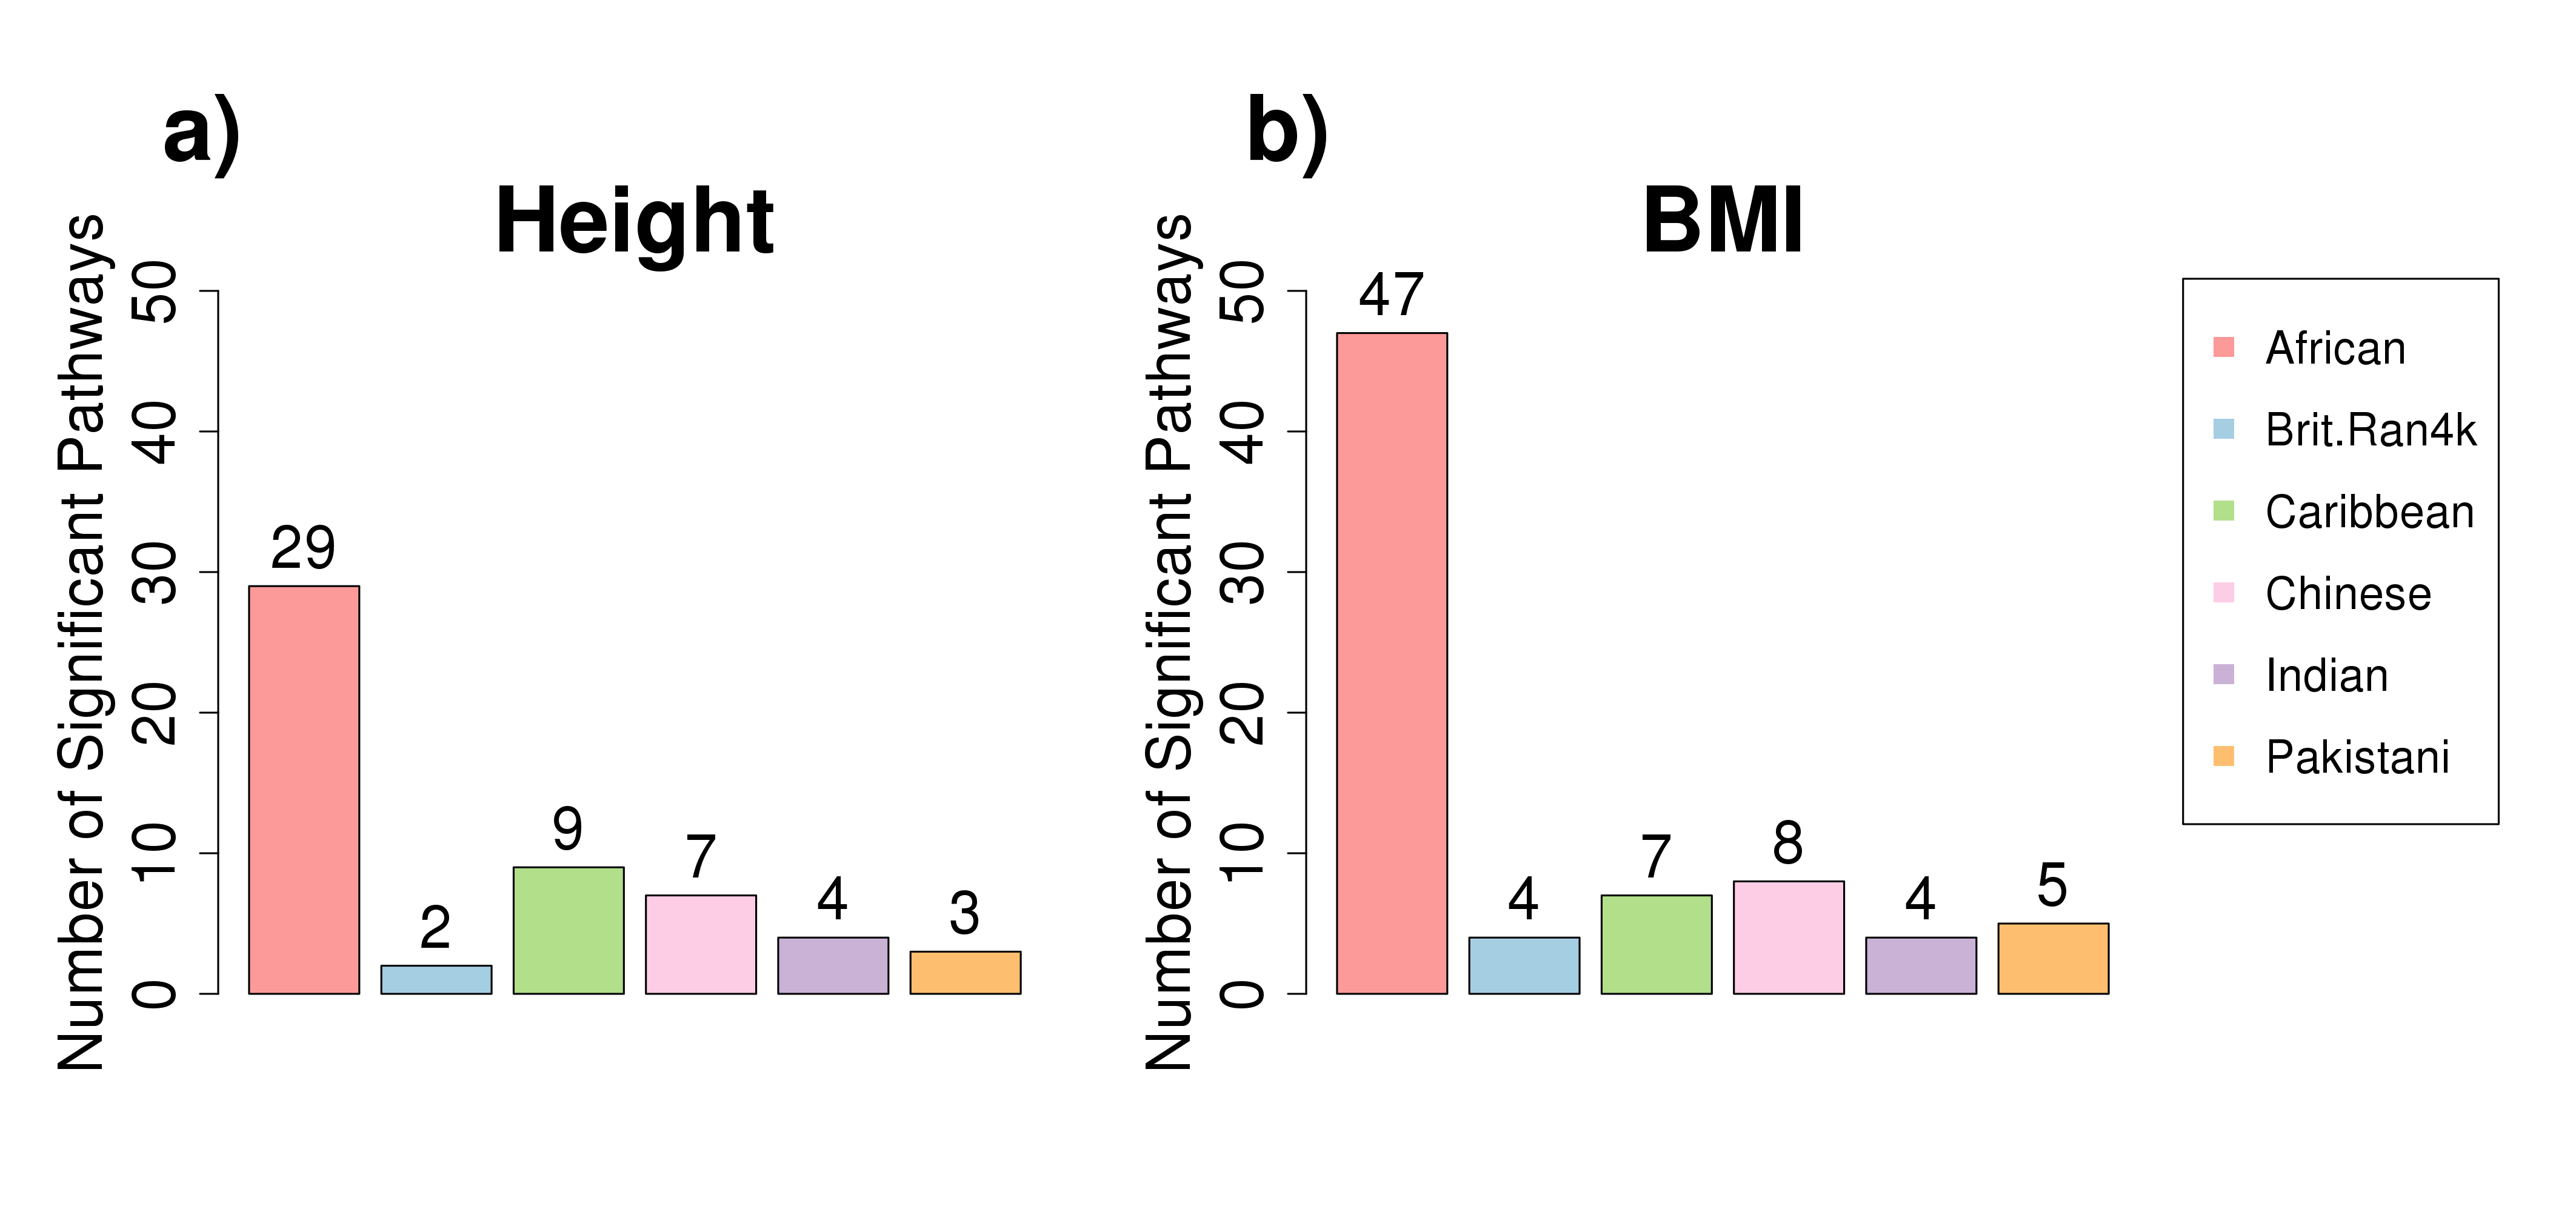
\includegraphics[width=\textwidth]{Images/Main/Figure1.png}
\caption{\textbf{Number of KEGG pathways identified by MAPIT-R that have significant marginal epistatic effects within (a) standing height and (b) body mass index (BMI) per subgroup in the UK Biobank.} Here, subgroups in the UK Biobank included individuals based on their self-identified ancestries: ``African'', ``British'', ``Caribbean'', ``Chinese'', ``Indian'', and ``Pakistani'' (see legend to the right of panel \textbf{(b)}). Genome-wide significance was determined by using Bonferroni-corrected $p$-value thresholds based on the number of pathways tested in each database-phenotype-subgroup combination (see Supplementary Table \ref{MAPITR-Supp-Table-UKBPopStats}). Across all database-phenotype combinations, the African subgroup has the largest numbers of significant pathways. For lists of the specific significant pathways per database-phenotype-subgroup combination, see Supplementary Table \ref{MAPITR-Supp-Table-TopPathways}. Results from running MAPIT-R with REACTOME database pathways can be found in Supplementary Figure \ref{MAPITR-Supp-Figure-Barplots-REACTOME}.}
\label{MAPITR-Main-Figure-Barplots-KEGG}
\end{figure}

%%%%%%%%%%%%%%%%%%%%%%%%%%%%%%%%%%%%%%%%%%%%%%%%%%%

\begin{landscape}
\begin{table}[htbp]
\centering
\hspace*{-8.25em}
\vspace*{-4em}
\resizebox{1.3\columnwidth}{!}{ \begin{tabular}{|c|c|ccc|ccc|}
  \hline
   \multirow{3.5}{*}{\textbf{Biological Category}} &
   \multirow{3.75}{*}{\shortstack{\textbf{KEGG Pathway} \\ \textbf{Annotation}}} &
   \multicolumn{3}{c|}{\multirow{1.25}{*}{\textbf{Height}}} &
   \multicolumn{3}{c|}{\multirow{1.25}{*}{\textbf{BMI}}} \\[2pt]
   \cline{3-5} \cline{6-8}
   & & \multirow{2.5}{*}{\shortstack{\textbf{MAPIT-R}\\ \textbf{$p$-Value}}} & \multirow{2.5}{*}{\shortstack{\textbf{Highlighted} \\ \textbf{Genes}}} & \multirow{2.5}{*}{\textbf{References}} & \multirow{2.5}{*}{\shortstack{\textbf{MAPIT-R}\\ \textbf{$p$-Value}}}  & \multirow{2.5}{*}{\shortstack{\textbf{Highlighted} \\ \textbf{Genes}}} & \multirow{2.5}{*}{\textbf{References}} \\[16pt]
\hline

 \multirow{9}{*}{\textbf{Cellular Signaling}}
 
 & \multirow{2}{*}{\texttt{CHEMOKINE\_SIGNALING\_PATHWAY}} & \multirow{2}{*}{$5.14\times 10^{-10}$} & \multirow{2.5}{*}{\shortstack{\textit{PCSK5}, \textit{CDC42EP3}, \\ \textit{STAT2}}} & \multirow{2}{*}{\cite{He2015,Tachmazidou2017,Akiyama2019}} & \multirow{2}{*}{$1.51\times 10^{-8}$} & \multirow{2.5}{*}{\shortstack{\textit{ADCY3}, \\\textit{PLCB3}}} & \multirow{2}{*}{\cite{Saeed2018,Cao2020}} \\[16pt]
 
 & \multirow{2}{*}{\texttt{CYTOKINE\_CYTOKINE\_RECEPTOR\_INTERACTION}} & \multirow{2}{*}{$2.84\times 10^{-8}$} & \multirow{2}{*}{\shortstack{\textit{GDF5}, \textit{LTBP1},\\\textit{LTBP2}}} & \multirow{2}{*}{\cite{Wood2014a,Kichaev2019,Wojcik2019}} & \multirow{2}{*}{NS} & \multirow{2}{*}{NS} & \multirow{2}{*}{NS} \\[16pt]
 
 & \multirow{2}{*}{\texttt{WNT\_SIGNALING\_PATHWAY}} & \multirow{2}{*}{$6.54\times 10^{-6}$} & \multirow{2}{*}{\shortstack{\textit{FBXW11}, \textit{NFATC4},\\\textit{ANAPC10}}} & \multirow{2}{*}{\cite{Berndt2013,Akiyama2019,Kichaev2019}} & \multirow{2}{*}{$1.41\times 10^{-7}$} & \multirow{2}{*}{\shortstack{\textit{CEP63}, \textit{ANAPC13},\\\textit{SMAD3}}} & \multirow{2}{*}{\cite{Shungin2015,Graff2017,Pulit2019}} \\[16pt]
 
 & \multirow{2}{*}{\texttt{ERBB\_SIGNALING\_PATHWAY}} & \multirow{2}{*}{NS} & \multirow{2}{*}{NS} & \multirow{2}{*}{NS} & \multirow{2}{*}{$3.30\times 10^{-7}$} & \multirow{2}{*}{\shortstack{\textit{VEGFA}, \textit{MACROD1},\\\textit{ERBB4}}} & \multirow{2}{*}{\cite{Lotta2018,Justice2019,Zhu2020}} \\ [14pt]\hline
 
  \multirow{6.5}{*}{\textbf{Immune System}} 
  & \multirow{2}{*}{\texttt{AUTOIMMUNE\_THYROID\_DISEASE}} & \multirow{2}{*}{$1.49\times 10^{-6}$} & \multirow{2.5}{*}{\shortstack{\textit{TGFB2},\\ \textit{HLA-C}}} & \multirow{2}{*}{\cite{Akiyama2019,Wojcik2019}} &  \multirow{2}{*}{$1.39\times 10^{-8}$} & \multirow{2.5}{*}{\shortstack{\textit{LYPLAL1}, \textit{ITGB8},\\ \textit{HLA-DRB1}}} & \multirow{2}{*}{\cite{Chu2017,Graff2017,Zhu2020}} \\[16pt]
  
  & \multirow{2}{*}{\texttt{ALLOGRAFT\_REJECTION}} & \multirow{2}{*}{$8.15\times 10^{-8}$} & \multirow{2}{*}{\shortstack{\textit{HLA-B},\\\textit{HLA-C}}} & \multirow{2}{*}{\cite{Wood2014a,Akiyama2019}} & \multirow{2}{*}{$2.53\times 10^{-8}$} & \multirow{2}{*}{\shortstack{\textit{TNFAIP8}, \textit{HSD17B4},\\\textit{DTWD2}}} & \multirow{2}{*}{\cite{Shungin2015,Winkler2015,Zhu2020}} \\[16pt]
  
  & \multirow{2}{*}{\texttt{ANTIGEN\_PROCESSING\_AND\_PRESENTATION}} & \multirow{2}{*}{$2.89\times 10^{-5}$} & \multirow{2}{*}{\shortstack{\textit{C2CD4A},\\\textit{HLA-B}}} & \multirow{2}{*}{\cite{Lango2010,Akiyama2019}} & \multirow{2}{*}{$2.08\times 10^{-7}$} & \multirow{2}{*}{\shortstack{\textit{IFI30}, \textit{ZNF318},\\\textit{TJAP1}}} & \multirow{2}{*}{\cite{Winkler2015,Justice2019}}\\ [14pt]\hline
  
  \multirow{4.5}{*}{\textbf{Heart Condition}} 
  & \multirow{2}{*}{\texttt{DILATED\_CARDIOMYOPATHY}} & \multirow{2}{*}{$1.24\times 10^{-7}$} & \multirow{2.5}{*}{\shortstack{\textit{IGF1}, \textit{IGF1R},\\\textit{POMC}}} & \multirow{2}{*}{\cite{Berndt2013,Kichaev2019,Wojcik2019}} & \multirow{2}{*}{$6.99\times 10^{-6}$} & \multirow{2.5}{*}{\shortstack{\textit{TGFB2}, \textit{ADCY3},\\\textit{HSD17B4}}} & \multirow{2}{*}{\cite{Shungin2015,Saeed2018,Zhu2020}} \\[16pt]
  
  & \multirow{2}{*}{\texttt{VIRAL\_MYOCARDITIS}} & \multirow{2}{*}{$1.89\times 10^{-5}$} & \multirow{2}{*}{\shortstack{\textit{HMGA1}, \textit{HLA-B},\\\textit{LAMA2}}} & \multirow{2}{*}{\cite{Wood2014a,Akiyama2019,Wojcik2019}} & \multirow{2}{*}{$1.09\times 10^{-6}$} & \multirow{2}{*}{\shortstack{\textit{HMGA1}, \textit{CYCSL1},\\\textit{HLA-DRB1}}} & \multirow{2}{*}{\cite{Graff2017,Zhu2020}} \\ [14pt]\hline
  
  \multirow{9}{*}{\textbf{Metabolism}} 
  & \multirow{2}{*}{\texttt{PURINE\_METABOLISM}} & \multirow{2}{*}{$1.19\times 10^{-7}$} & \multirow{2.5}{*}{\shortstack{\textit{ADAMTSL3}, \textit{ADAMTS17},\\\textit{PDE3A}}} & \multirow{2}{*}{\cite{Rueger2018,Akiyama2019,Kichaev2019}} & \multirow{2}{*}{$2.46\times 10^{-6}$} & \multirow{2.5}{*}{\shortstack{\textit{ADAMTSL3}, \textit{ADAMTS9},\\\textit{CENTA2}}} & \multirow{2}{*}{\cite{Justice2019,Zhu2020}} \\[16pt]
  
  & \multirow{2}{*}{\texttt{BETA\_ALANINE\_METABOLISM}} & \multirow{2}{*}{NS} & \multirow{2}{*}{NS} & \multirow{2}{*}{NS} & \multirow{2}{*}{$1.12\times 10^{-4}$} & \multirow{2}{*}{\shortstack{\textit{DPYSL5},\\ \textit{DPYD}}} & \multirow{2}{*}{\cite{Manning2012,Tachmazidou2017}} \\[16pt]
  
  & \multirow{2}{*}{\texttt{ETHER\_LIPID\_METABOLISM}} & \multirow{2}{*}{NS} & \multirow{2}{*}{NS} & \multirow{2}{*}{NS} & \multirow{2}{*}{$1.41\times 10^{-4}$} & \multirow{2}{*}{\shortstack{\textit{PLA2G6},\\\textit{PLA2G4A}}} & \multirow{2}{*}{\cite{Spracklen2017,Tachmazidou2017}} \\[16pt]
  
  & \multirow{2}{*}{\texttt{O\_GLYCAN\_BIOSYNTHESIS}} & \multirow{2}{*}{NS} & \multirow{2}{*}{NS} & \multirow{2}{*}{NS} & \multirow{2}{*}{$1.92\times 10^{-4}$} & \multirow{2}{*}{\shortstack{\textit{GALNT10},\\\textit{B4GALNT3}}} & \multirow{2}{*}{\cite{Ng2012,Zhu2020}} \\ [14pt]\hline
\end{tabular}}
\bigskip  \bigskip  \bigskip
  \caption{\textbf{Biological themes among the MAPIT-R significant KEGG pathways for height and body mass index (BMI) within the African subgroup in the UK Biobank}. The biological themes include: cellular signaling, immune system, heart condition, and metabolism. Notably enriched pathways for each biological theme are included in the second column. For each pathway, MAPIT-R $p$-values, highlighted gene associations, and references for each gene association are shown for both height (third, forth, and fifth columns) and BMI (sixth, seventh, and eighth columns). Genome-wide significance was determined by using Bonferroni-corrected $p$-value thresholds based on the number of pathways tested in each database-phenotype-subgroup combination (Supplementary Table \ref{MAPITR-Supp-Table-UKBPopStats}). ``Highlighted Genes'' and ``References'' were determined using relevant SNP association citations from the GWAS Catalog (version 1.0.2) \cite{Buniello2019}. For a full list of MAPIT-R significant pathways in all database-phenotype-subgroup combinations, see Supplementary Table \ref{MAPITR-Supp-Table-TopPathways}. NS indicates that a pathway was not genome-wide significant for a given phenotype.}
\label{MAPITR-Main-Table-KEGG-African-TopPathways-Themes}
\end{table}
\end{landscape}

%%%%%%%%%%%%%%%%%%%%%%%%%%%%%%%%%%%%%%%%%%%%%%%%%%%

\begin{figure}[htb]
\centering
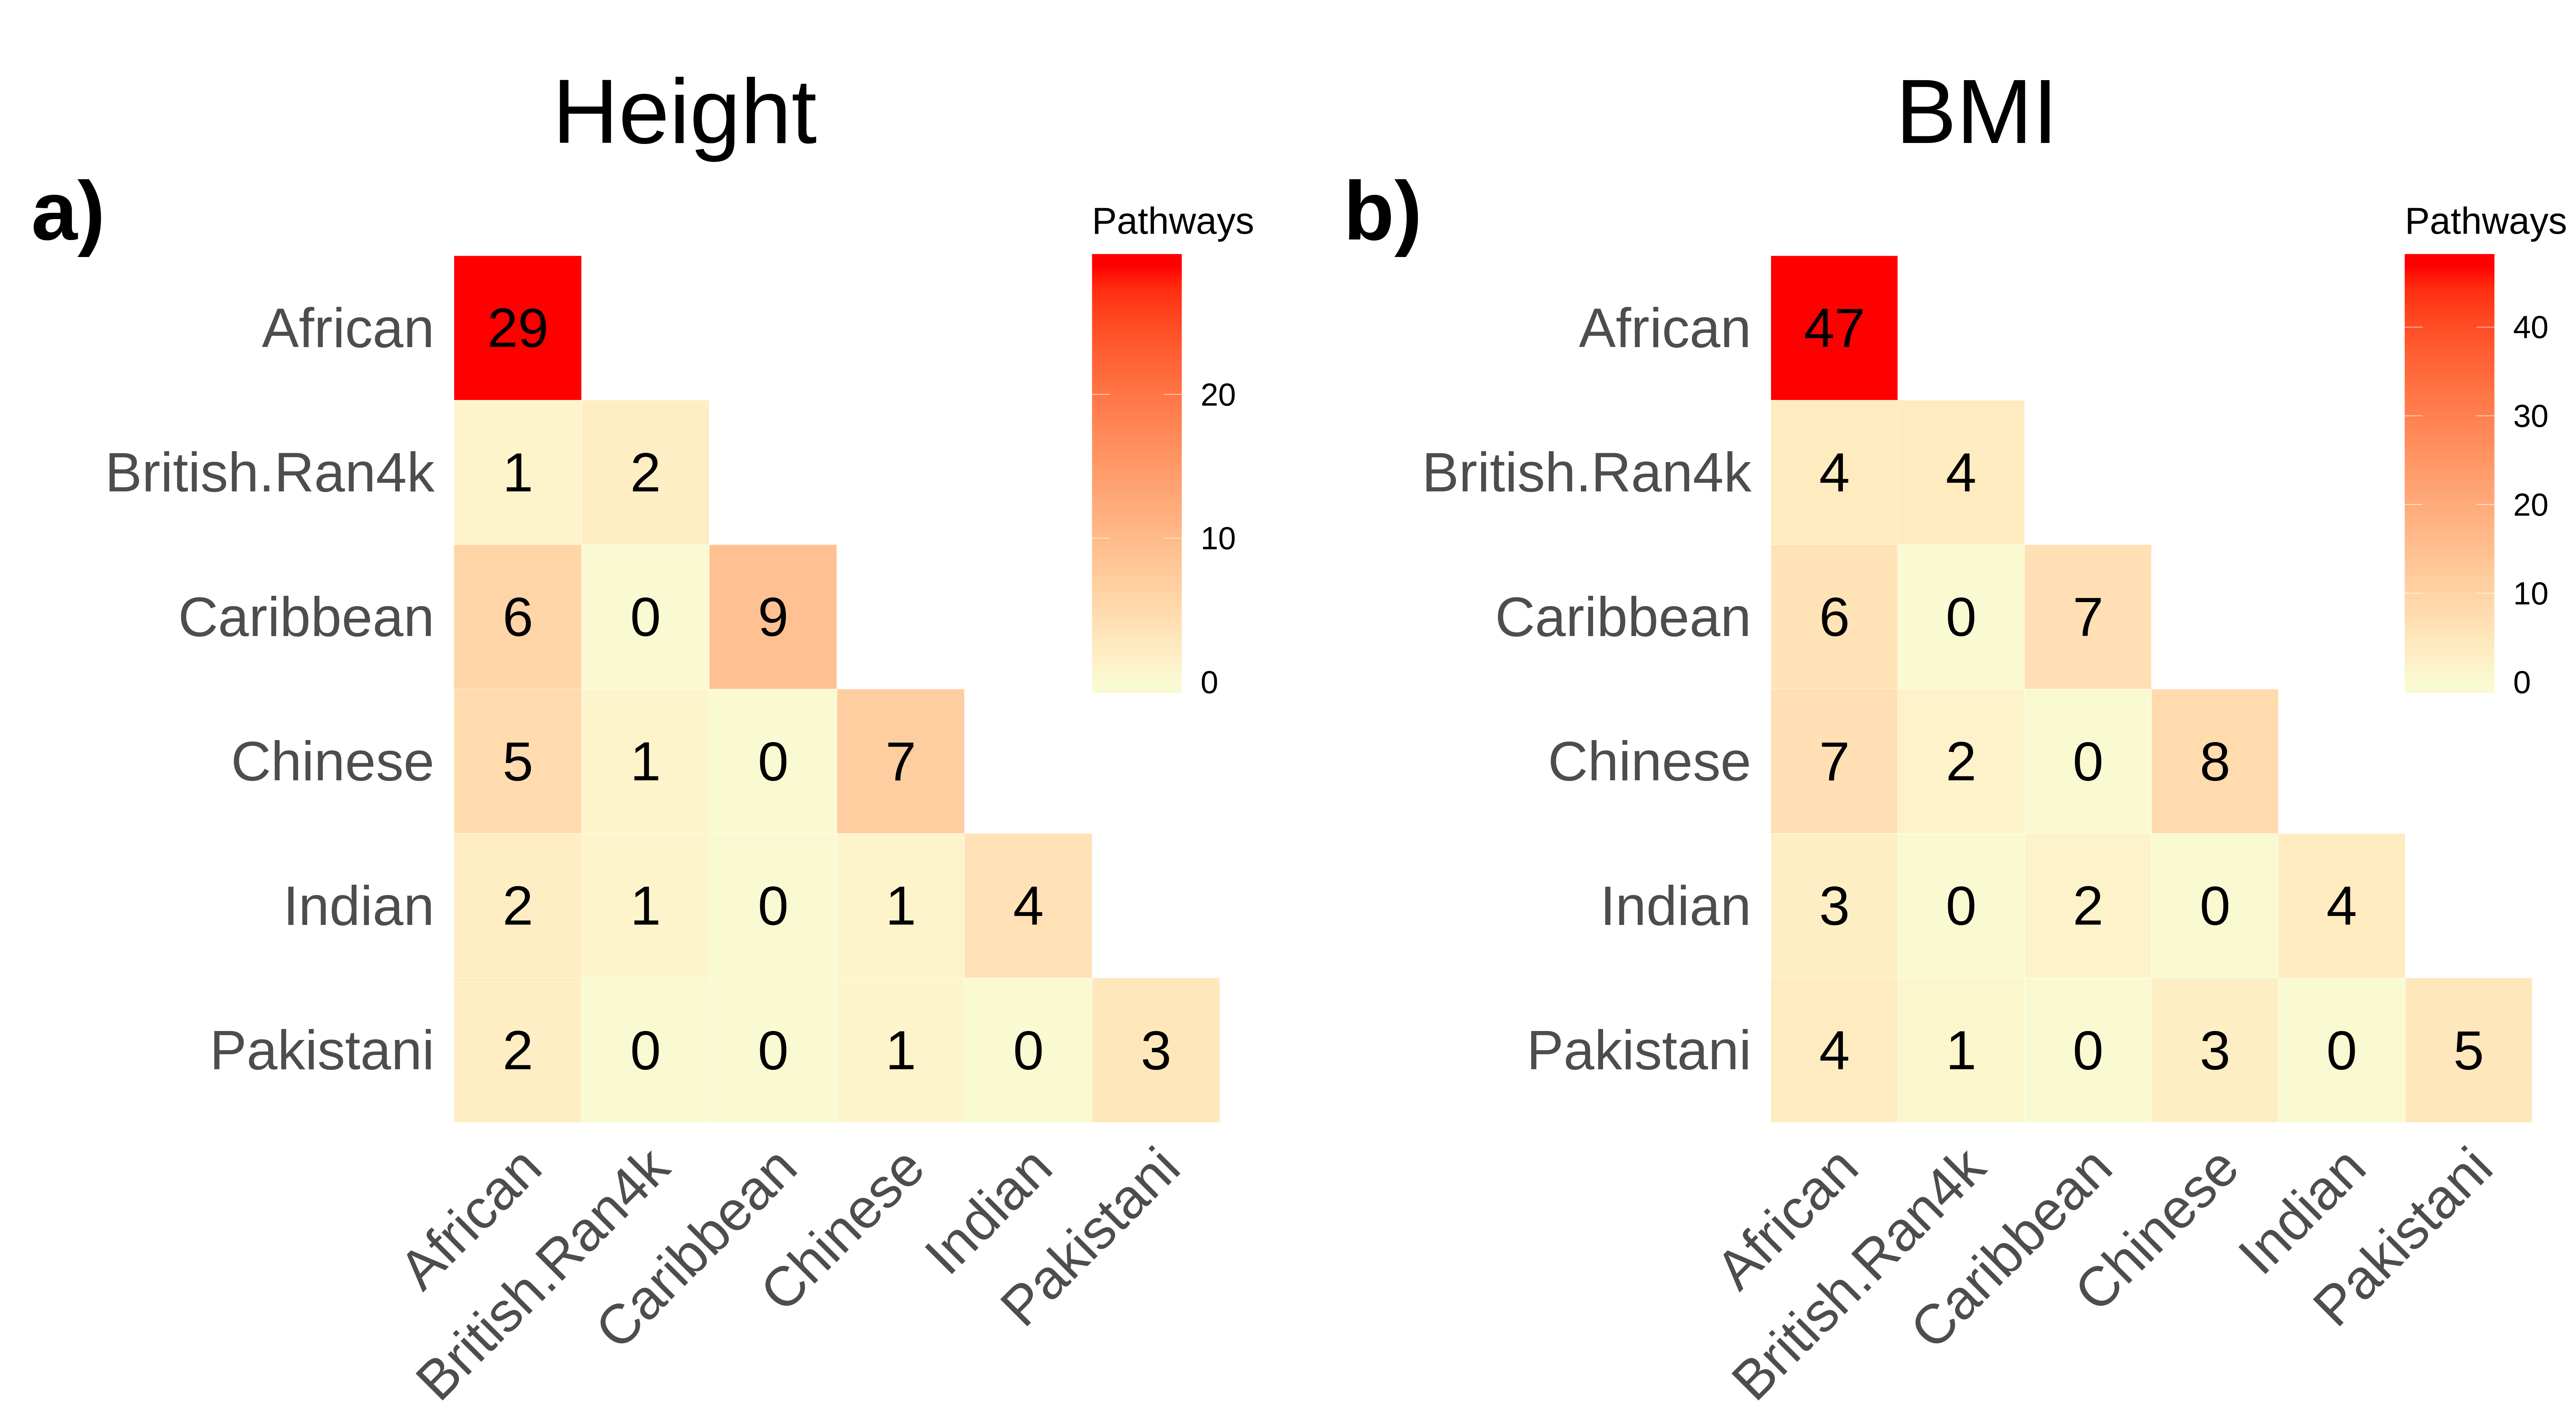
\includegraphics[width=\textwidth]{Images/Main/Figure2.png}
\caption{\textbf{Heatmaps depicting the overlap of MAPIT-R significant KEGG pathways for (a) standing height and (b) body mass index (BMI) across the different ancestry-specific subgroups in the UK Biobank}. Here, subgroups in the UK Biobank included individuals based on their self-identified ancestries: ``African'', ``British'', ``Caribbean'', ``Chinese'', ``Indian'', and ``Pakistani'' (ordered here from top-to-bottom and left-to-right). Genome-wide significance was determined by using Bonferroni-corrected $p$-value thresholds based on the number of pathways tested in each database-phenotype-subgroup combination (see Supplementary Table \ref{MAPITR-Supp-Table-UKBPopStats}). The diagonal shows the total number of genome-wide significant pathways per subgroup. We observe that significant pathways identified in non-African subgroups overlap more often with pathways from the African subgroup than they do with pathways from the other, remaining non-African subgroups. Results for both phenotypes in the REACTOME database can be seen in Supplementary Figure \ref{MAPITR-Supp-Figure-Heatplots-REACTOME}.}
\label{MAPITR-Main-Figure-Heatplots-KEGG}
\end{figure}

%%%%%%%%%%%%%%%%%%%%%%%%%%%%%%%%%%%%%%%%%%%%%%%%%%%

\begin{figure}[htb]
\centering
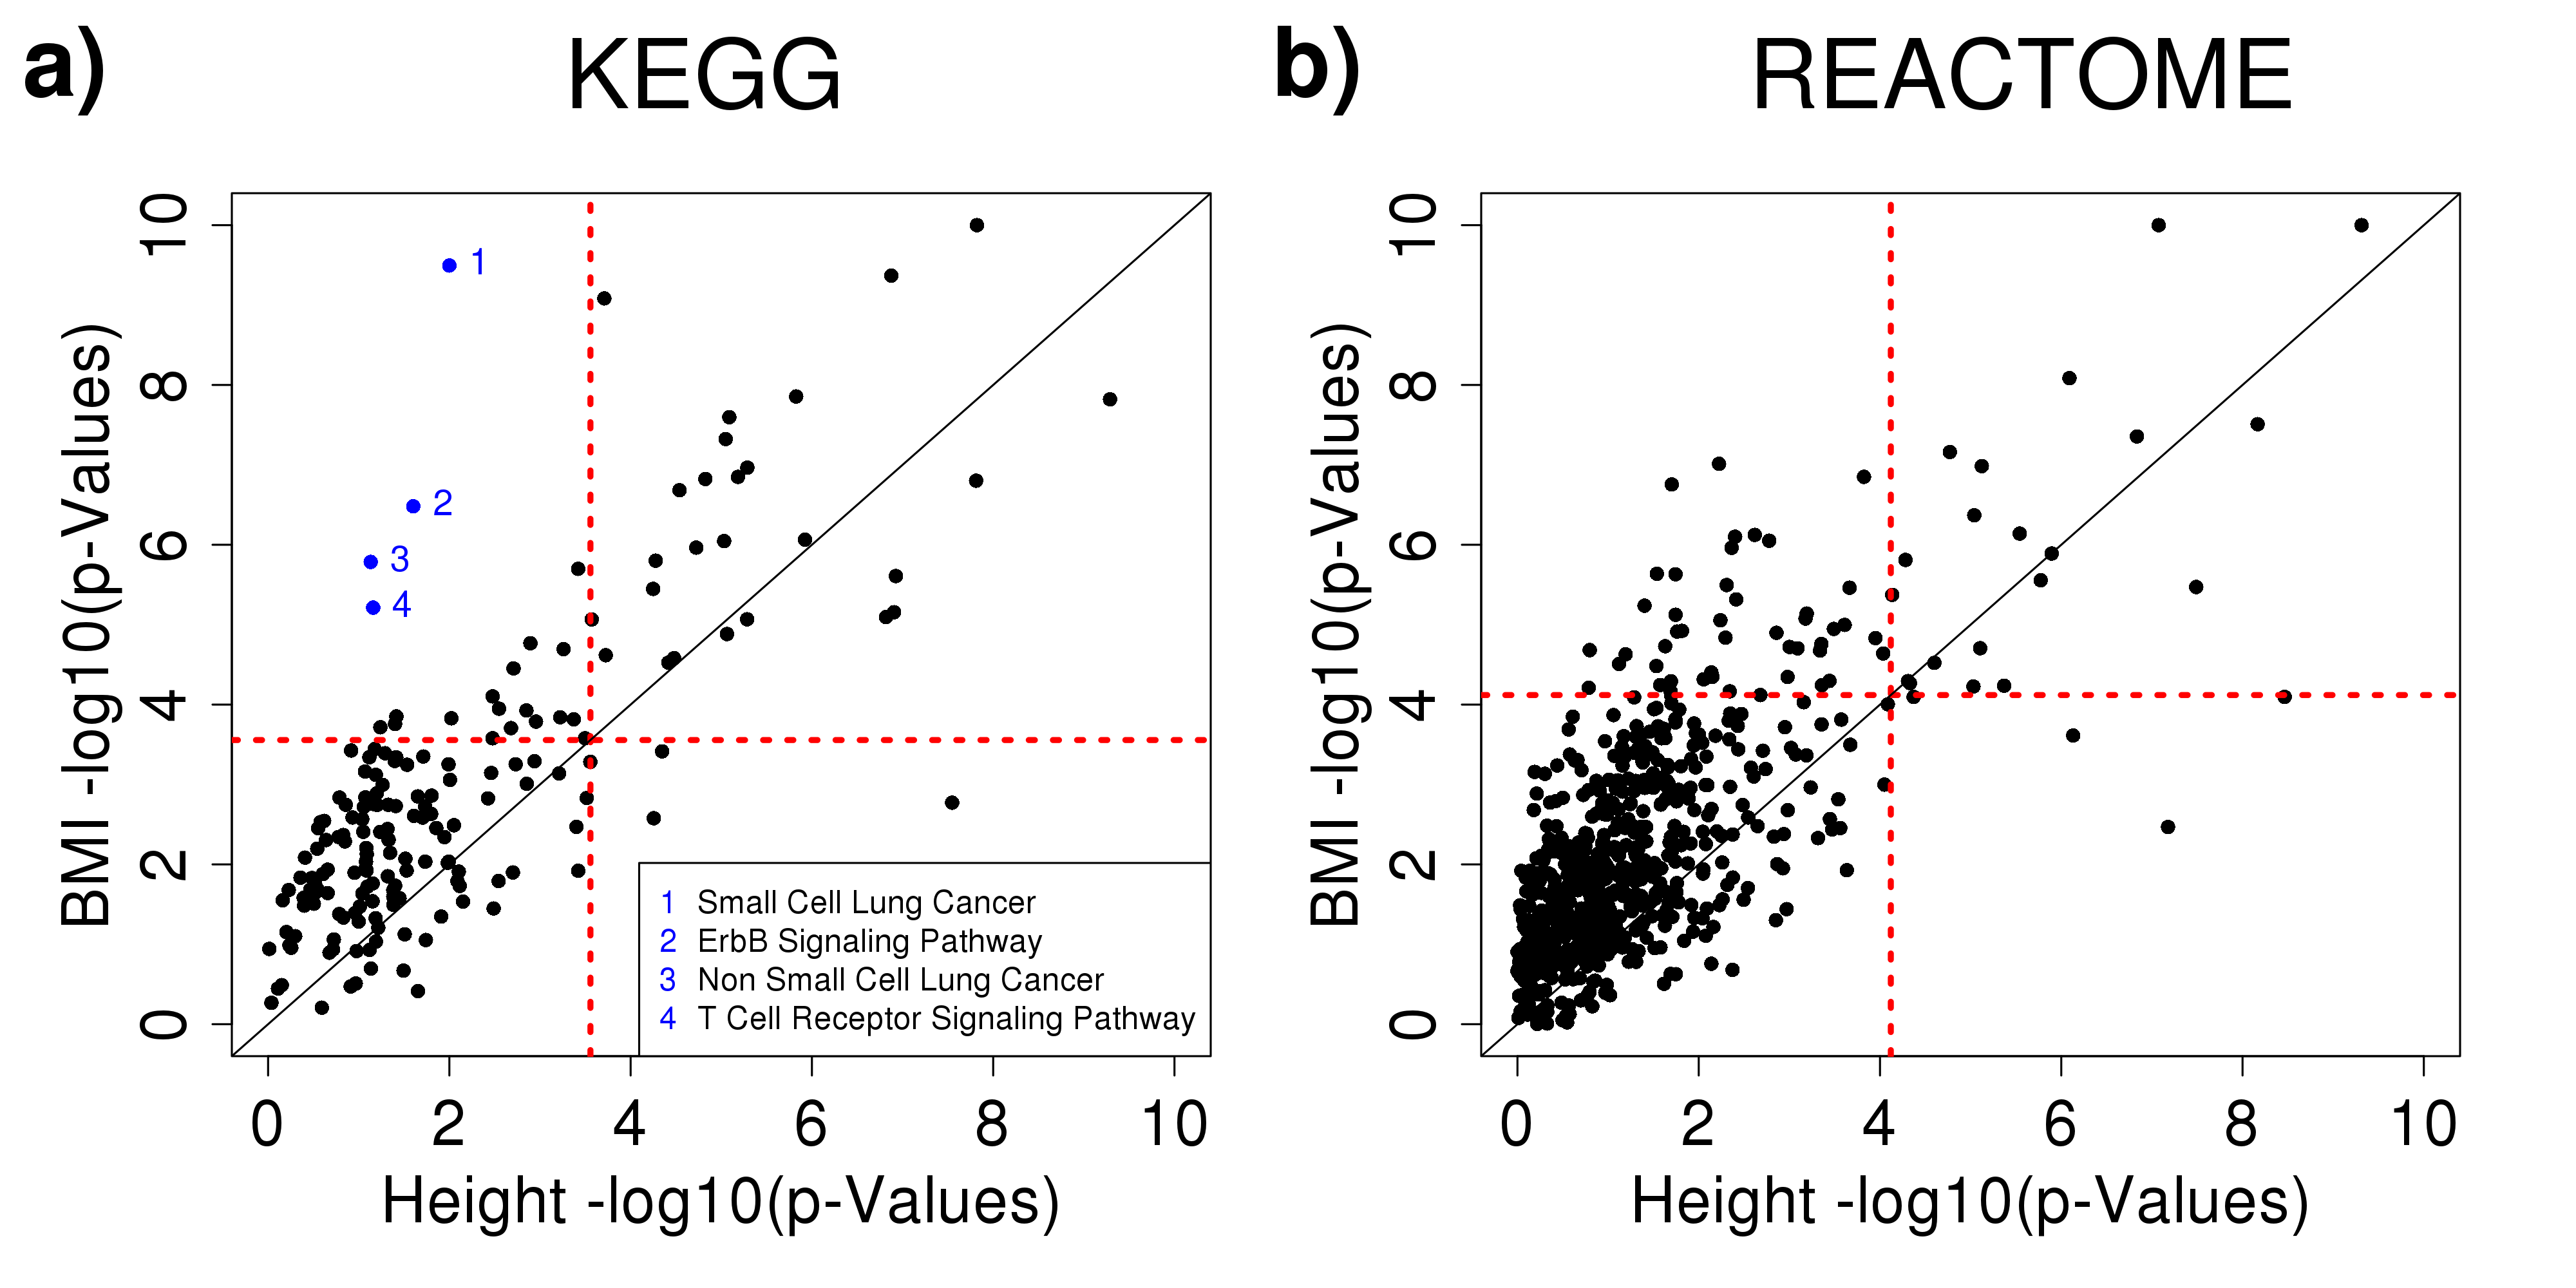
\includegraphics[width=\textwidth]{Images/Main/Figure3.png}
\caption{\textbf{Scatterplots comparing the MAPIT-R $\bm{p}$-values using (a) KEGG and (b) REACTOME pathways annotations in height and body mass index (BMI) within the African subgroup in the UK Biobank.} For each plot, the $x$-axis shows the -$\log_{10}$ transformed MAPIT-R $p$-value for height, while the $y$-axis shows the same results for BMI. The red horizontal and vertical dashed lines are marked at the Bonferroni-corrected $p$-value thresholds for genome-wide significance in each pathway-phenotype combination (see Supplementary Table \ref{MAPITR-Supp-Table-UKBPopStats}). Pathways in the top right quadrant have significant marginal epistatic effects in both traits; while, points in the bottom right and top left quadrants are pathways that are uniquely enriched in height or BMI, respectively. The four highlighted pathways in blue represent a cluster of oncogenic and signaling pathways whose loci have been functionally connected to BMI in previous studies \cite{George2004,Ortega-Molina2015,Manning2017,Justice2017,Latva-Rasku2018,Grigsby2018,Huang2018,Couto2019}. Across both databases, BMI results have lower MAPIT-R $p$-values than height results on average. For these comparisons in all of the UK Biobank subgroups, see Supplementary Figure \ref{MAPITR-Supp-Figure-PhenoComps-AllPops}.}
\label{MAPITR-Main-Figure-PhenoComps-African}
\end{figure}

%%%%%%%%%%%%%%%%%%%%%%%%%%%%%%%%%%%%%%%%%%%%%%%%%%%

\begin{figure}[htb]
\centering
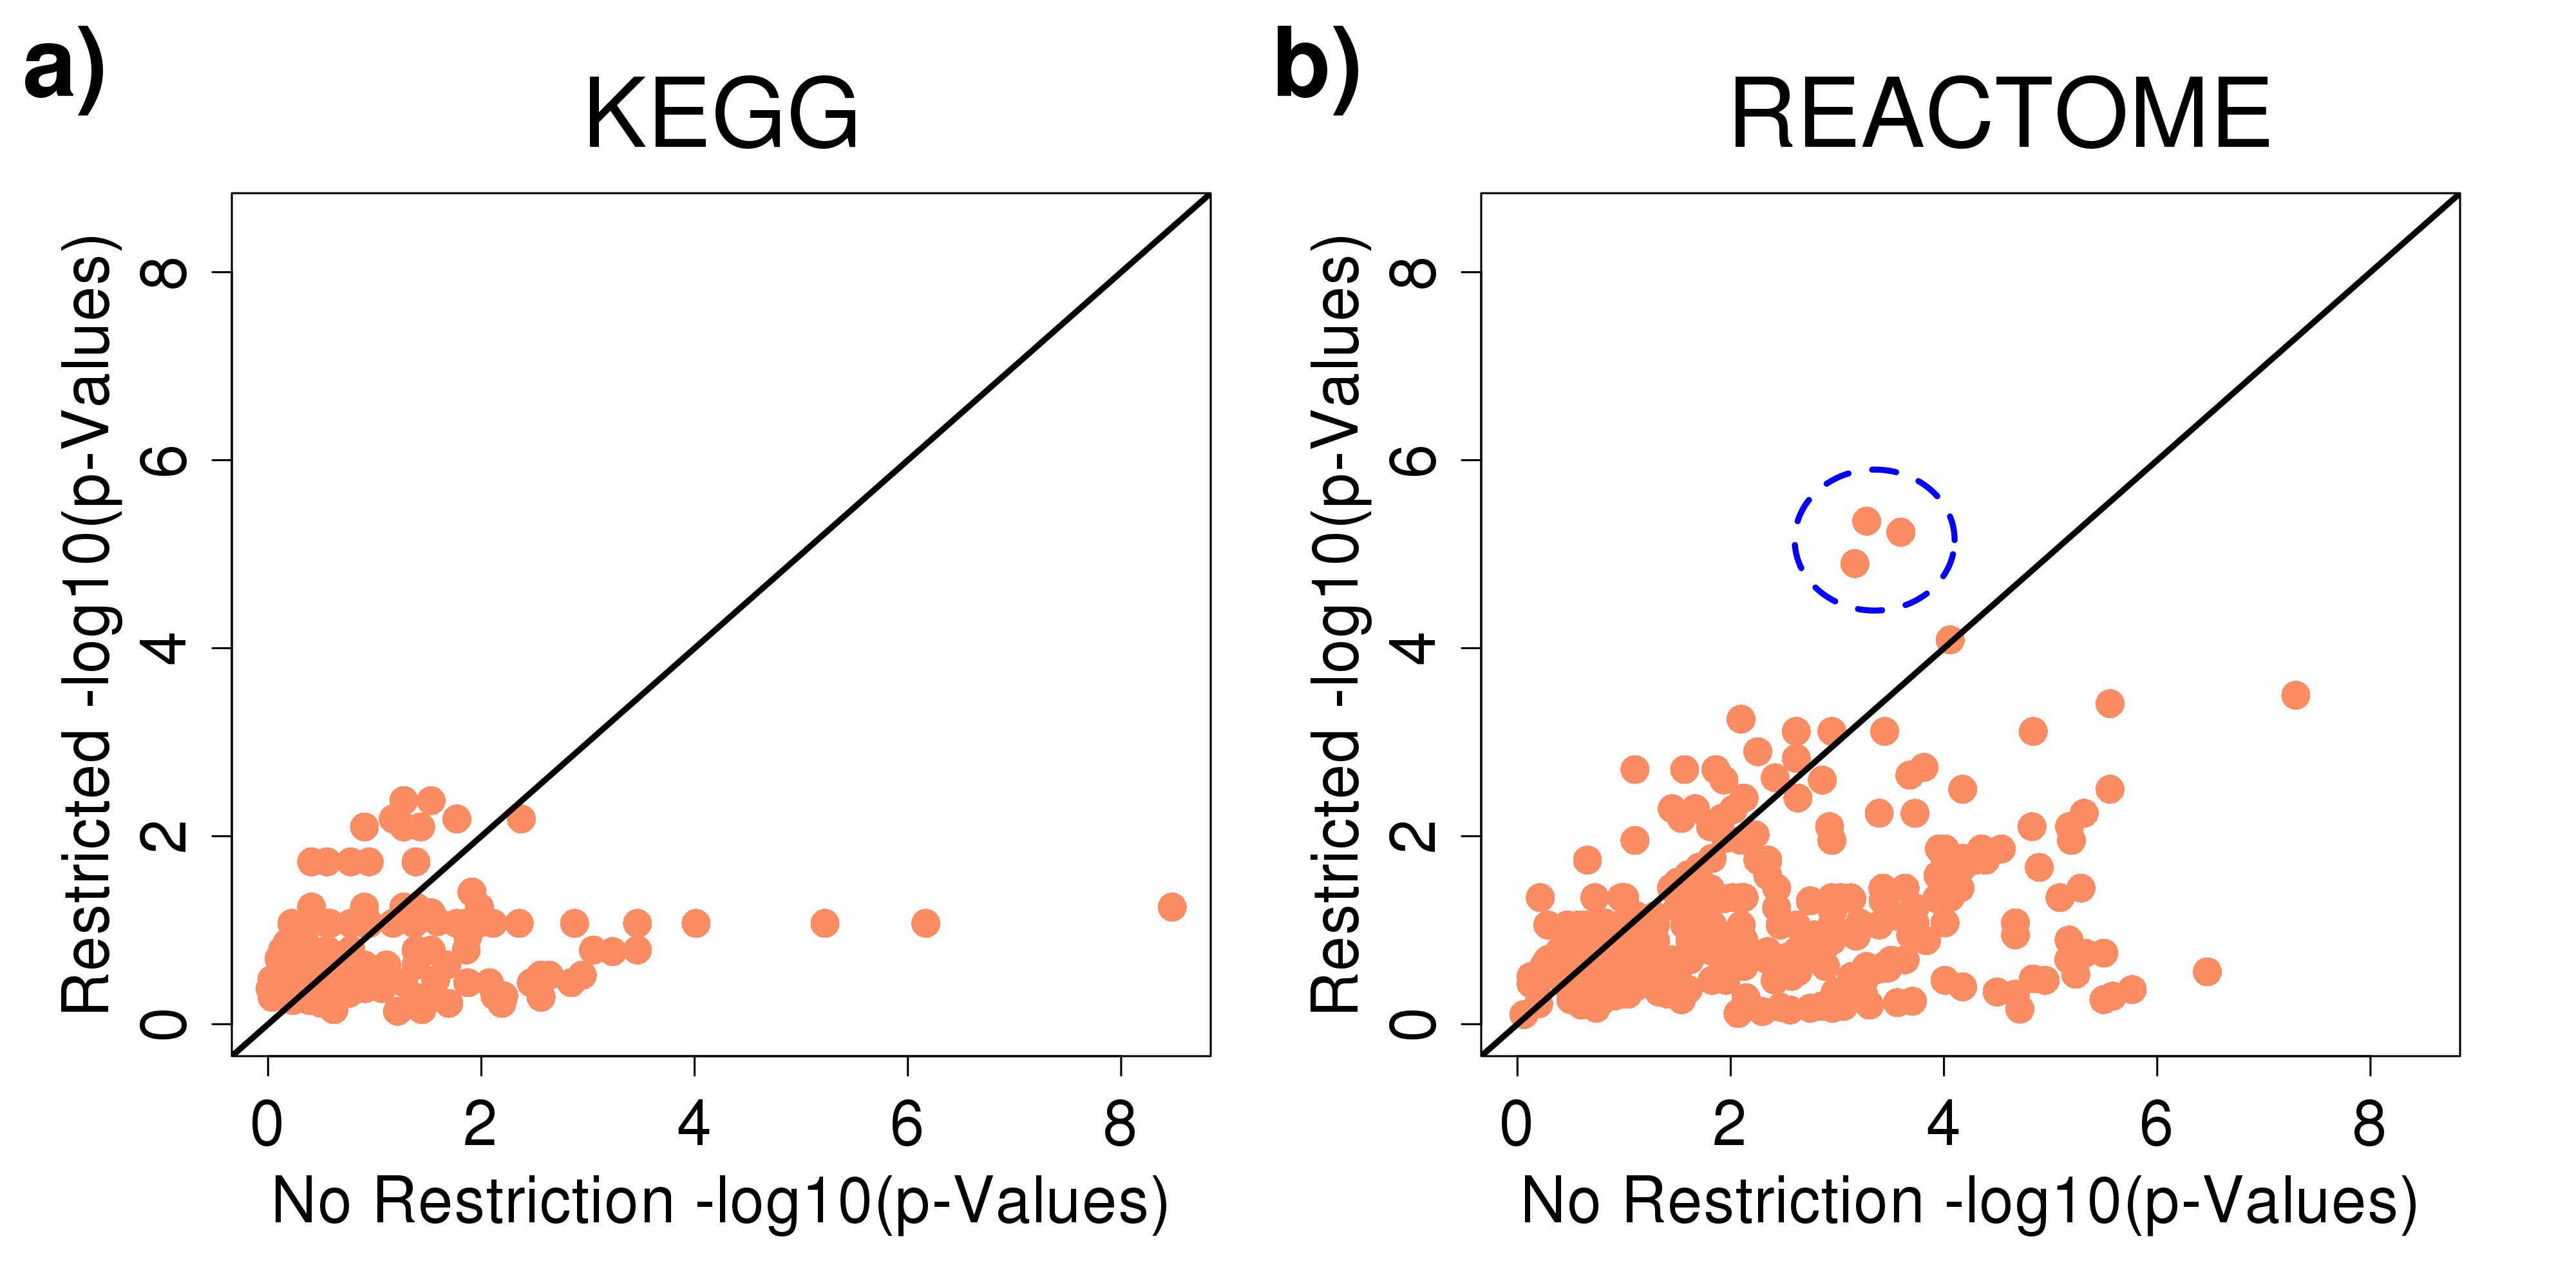
\includegraphics[width=\textwidth]{Images/Main/Figure4.png}
\caption{\textbf{Scatterplots comparing the $\bm{p}$-values from the hypergeometric enrichment analyses using only (a) KEGG and (b) REACTOME pathways annotations with at most 1000 SNPs within the African subgroup in the UK Biobank.} Here, the gene-based $p$-values using the size restricted pathways are shown on the $y$-axis, while the results from the original unrestricted version of the analysis are shown on the $x$-axis. The blue dashed circle in panel \textbf{(b)} highlights the proteasome gene family cluster. For lists containing each gene's original and size-restricted hypergeometric $p$-values, see Supplementary Table \ref{MAPITR-Supp-Table-Hypergeometric-RestrictedComps-African-BMI}. Note that we only show results for BMI because few MAPIT-R significant pathways in the height analysis remained after imposing the size restriction. For lists containing gene counts for each database-phenotype-subgroup combination under both the original and size-restricted data sets, see Supplementary Tables \ref{MAPITR-Supp-Table-TopGeneCounts} and \ref{MAPITR-Supp-Table-TopGeneCounts-SizeRestricted}.}
\label{MAPITR-Main-Figure-Hypergeometric-RestrictedComps-African-BMI}
\end{figure}

%%%%%%%%%%%%%%%%%%%%%%%%%%%%%%%%%%%%%%%%%%%%%%%%%%%

\begin{landscape}
\begin{figure}[htbp]
\centering
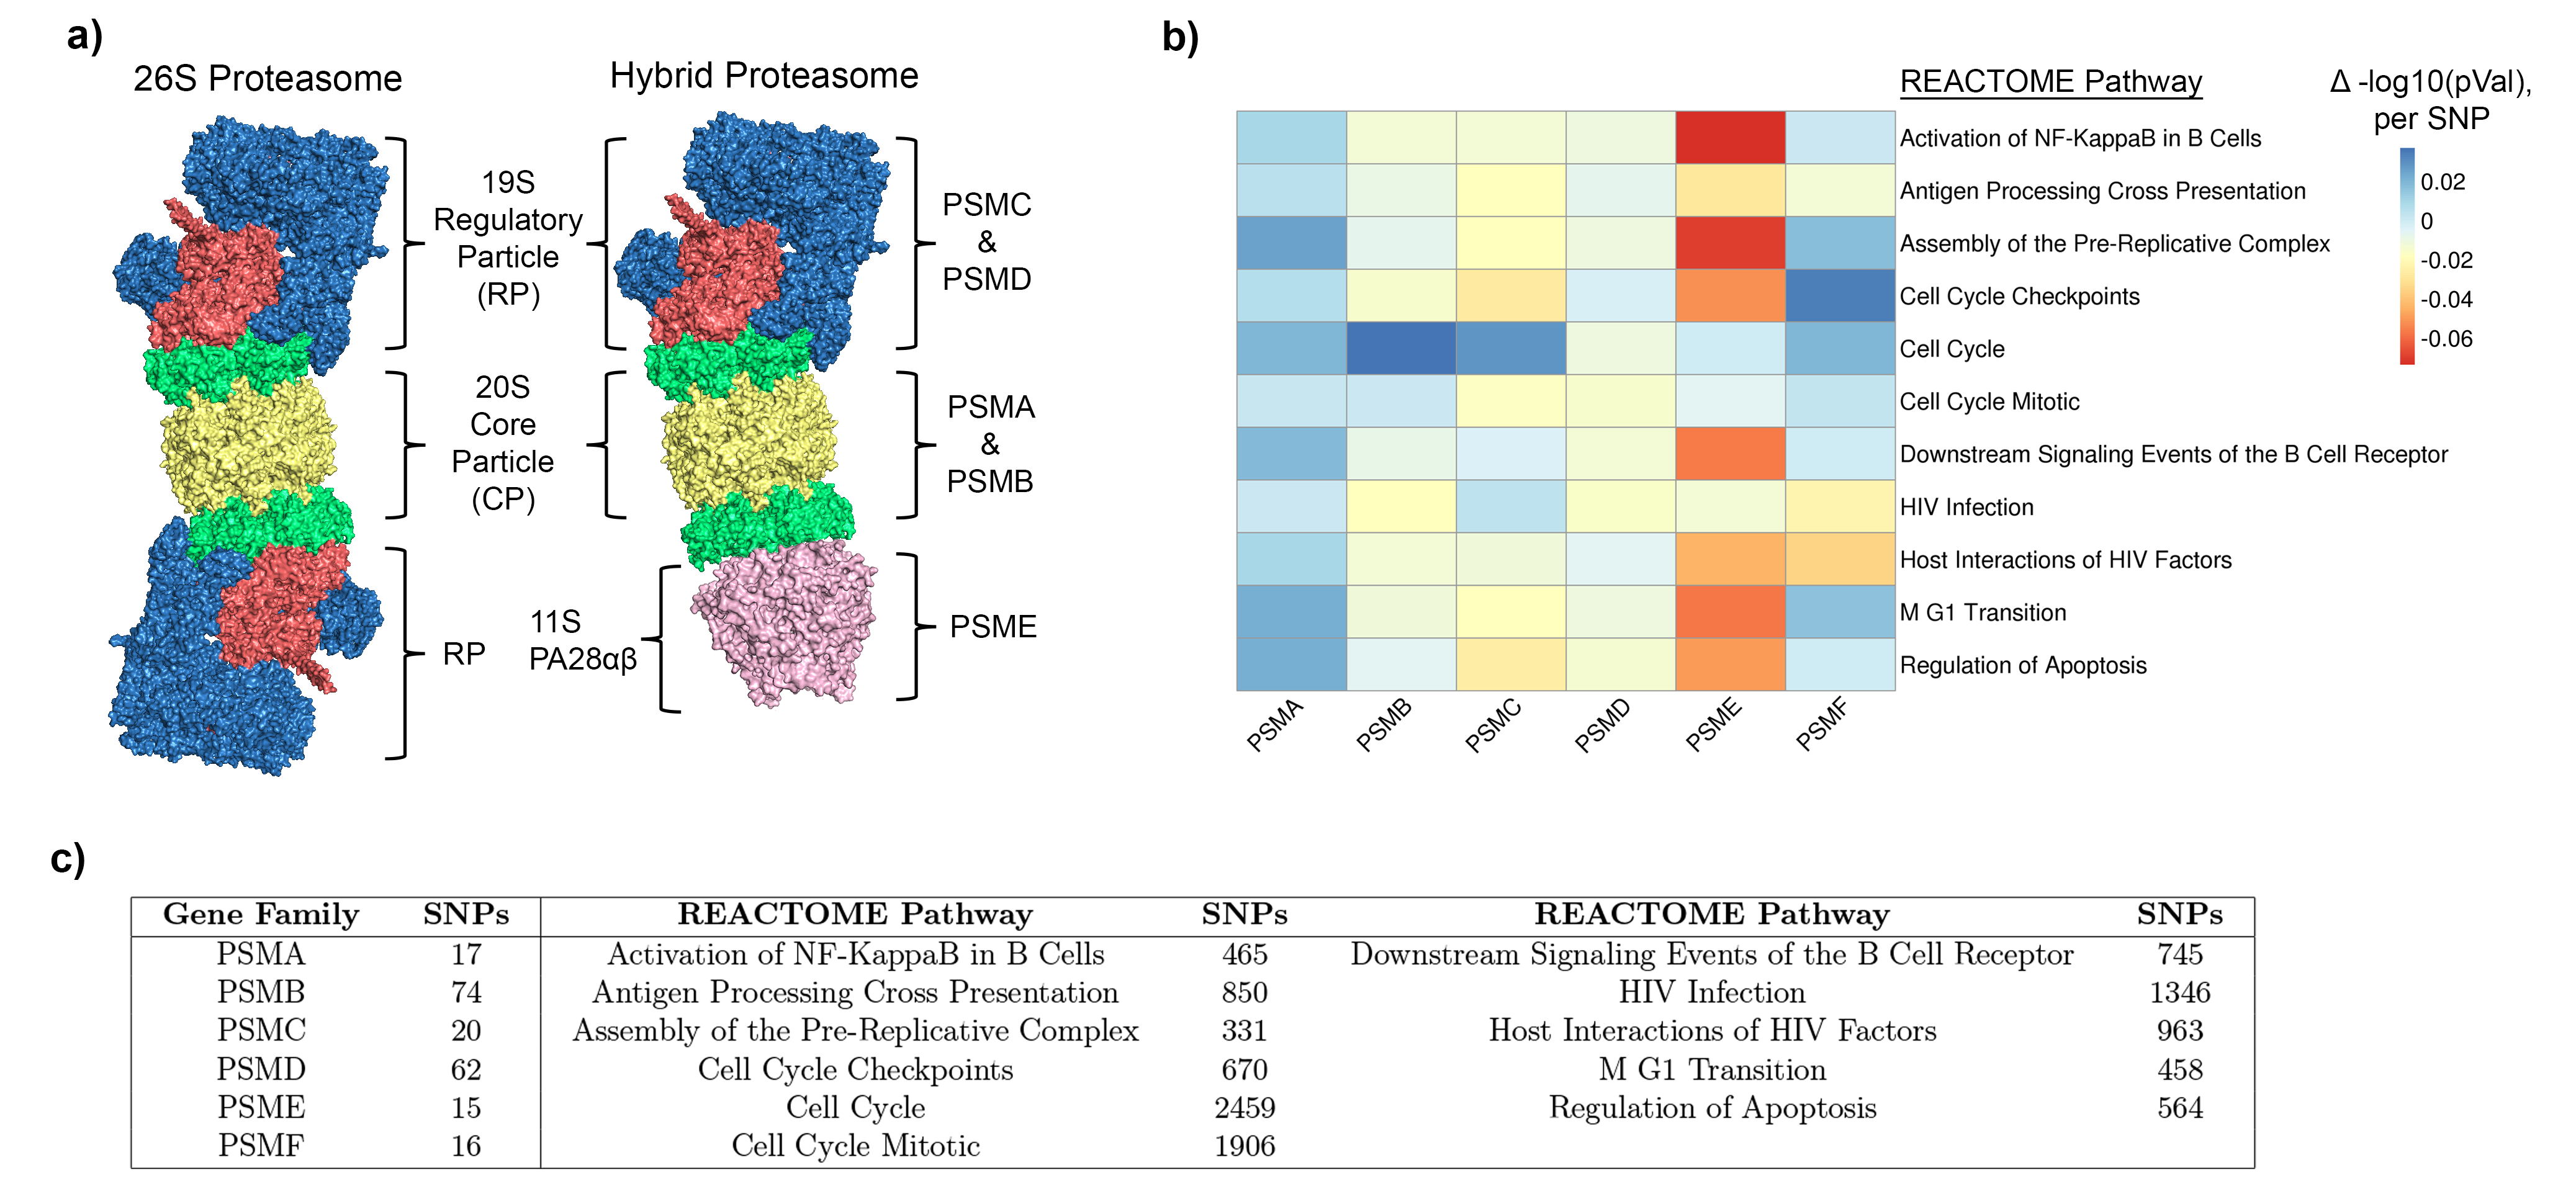
\includegraphics[scale=.6]{Images/Main/Figure5.png}
\caption{\textbf{Structure of the proteasome and results from applying a ``leave-one-out'' approach to MAPIT-R with proteasome gene families}. \textbf{(a)} Models of different isoforms of the proteasome, a complex protein structure required for proper degradation of many proteins in the cell. The ``26S Proteasome'' is the main isoform, composed of the 20S core particle (CP) and capped on both ends by the 19S regulatory particle (RP). The ``Hybrid Proteasome'' isoform is produced when the CP binds on one end with an RP and on the other end with the IFN-$\gamma$-inducible 11S complex PA28$\alpha\beta$. The \textit{PSMA} and \textit{PSMB} gene families encode components of the CP, the \textit{PSMC} and \textit{PSMD} gene families encode components of the RP, and members of the \textit{PSME} gene family encode PA28$\alpha\beta$. Note that \textit{PSMF} represents a proteasome inhibitor and is not shown. The structures shown were adopted and modified from the Protein Data Bank (human 26S proteasome, \url{https://www.rcsb.org/structure/5GJR}; mouse PA28$\alpha\beta$, \url{https://www.rcsb.org/structure/5MX5}) \cite{Murata2018}. \textbf{(b)} The heatmap shows the change in original MAPIT-R -$\log_{10}$ $p$-value for different REACTOME pathways when each proteasome gene family is removed one at a time in a ``leave-one-out'' manner. The analyses were conducted in BMI for the African subgroup of the UK Biobank. The $x$-axis shows each proteasome gene family and the $y$-axis lists each REACTOME pathway. Each column has been scaled by the number of SNPs present in the given gene family and, as a result, the heatmap specifically shows the -$\log_{10}$ $p$-value change ($\Delta$ in legend) per SNP. \textbf{(c)} The table shows the number of SNPs present in each proteasome gene family (left), as well as the number of SNPs present in each REACTOME pathway (right).}
\label{MAPITR-Main-Figure-Proteasome-Panels}
\end{figure} 
\end{landscape}

%%%%%%%%%%%%%%%%%%%%%%%%%%%%%%%%%%%%%%%%%%%%%%%%%%%

\begingroup
\setstretch{1.0}
\bibliography{Main}
\endgroup

\end{document}

%%%%%%%%%%%%%%%%%%%%%%%%%%%%%%%%%%%%%%%%%%%%%%%%%%%